% !TeX program = pdflatex
\documentclass{grattan}\usepackage[]{graphicx}\usepackage[]{color}
%% maxwidth is the original width if it is less than linewidth
%% otherwise use linewidth (to make sure the graphics do not exceed the margin)
\makeatletter
\def\maxwidth{ %
  \ifdim\Gin@nat@width>\linewidth
    \linewidth
  \else
    \Gin@nat@width
  \fi
}
\makeatother

\definecolor{fgcolor}{rgb}{0.345, 0.345, 0.345}
\newcommand{\hlnum}[1]{\textcolor[rgb]{0.686,0.059,0.569}{#1}}%
\newcommand{\hlstr}[1]{\textcolor[rgb]{0.192,0.494,0.8}{#1}}%
\newcommand{\hlcom}[1]{\textcolor[rgb]{0.678,0.584,0.686}{\textit{#1}}}%
\newcommand{\hlopt}[1]{\textcolor[rgb]{0,0,0}{#1}}%
\newcommand{\hlstd}[1]{\textcolor[rgb]{0.345,0.345,0.345}{#1}}%
\newcommand{\hlkwa}[1]{\textcolor[rgb]{0.161,0.373,0.58}{\textbf{#1}}}%
\newcommand{\hlkwb}[1]{\textcolor[rgb]{0.69,0.353,0.396}{#1}}%
\newcommand{\hlkwc}[1]{\textcolor[rgb]{0.333,0.667,0.333}{#1}}%
\newcommand{\hlkwd}[1]{\textcolor[rgb]{0.737,0.353,0.396}{\textbf{#1}}}%
\let\hlipl\hlkwb

\usepackage{framed}
\makeatletter
\newenvironment{kframe}{%
 \def\at@end@of@kframe{}%
 \ifinner\ifhmode%
  \def\at@end@of@kframe{\end{minipage}}%
  \begin{minipage}{\columnwidth}%
 \fi\fi%
 \def\FrameCommand##1{\hskip\@totalleftmargin \hskip-\fboxsep
 \colorbox{shadecolor}{##1}\hskip-\fboxsep
     % There is no \\@totalrightmargin, so:
     \hskip-\linewidth \hskip-\@totalleftmargin \hskip\columnwidth}%
 \MakeFramed {\advance\hsize-\width
   \@totalleftmargin\z@ \linewidth\hsize
   \@setminipage}}%
 {\par\unskip\endMakeFramed%
 \at@end@of@kframe}
\makeatother

\definecolor{shadecolor}{rgb}{.97, .97, .97}
\definecolor{messagecolor}{rgb}{0, 0, 0}
\definecolor{warningcolor}{rgb}{1, 0, 1}
\definecolor{errorcolor}{rgb}{1, 0, 0}
\newenvironment{knitrout}{}{} % an empty environment to be redefined in TeX

\usepackage{alltt}

\usepackage{ocgx}

\title{Negative gearing and the capital gains discount}
\author{John Daley and Danielle Wood}

\YEAR{2015}
\MONTH{August}
\GrattanReportNumber{2015-5}

\addbibresource{bibliography.bib}
\addbibresource{bibliography2.bib} % r packages

\usepackage{booktabs}
\usepackage{amsmath}
\usepackage{siunitx} % for decimal points in tables
\sisetup{detect-all} % to ensure helvetica is used
\usepackage{longtable} % session info
\usepackage{tabularx}  % boxed tables
% \usepackage{flushend} % for flushed columns at end of chapters
\usepackage{makecell}

\renewcommand{\classification}{\normalfont\textbf{\textcolor{red}{DRAFT NO CIRC}}}
\usepackage{grfext}
\PrependGraphicsExtensions*{.pdf}

% \title{Negative gearing and the capital gains discount}
% \usepackage[normalem]{ulem}
% \newcommand\redsout{\bgroup\markoverwith{\textcolor{red}{\rule[0.5ex]{2pt}{3pt}}}\ULon}
% \author{\redsout{John Daley and Danielle Wood}}

\newcommand{\TBD}[1]{\textcolor{yellow}{#1}}
  
  
\newcommand\gao{Grattan analysis of}
\newcommand{\mpfootnotes}[1][1]{
  \renewcommand{\thempfootnote}{\thefootnote}
  \addtocounter{footnote}{-#1}
  \renewcommand{\footnote}{\stepcounter{footnote}\footnotetext[\value{footnote}]}
  }
    
\usetikzlibrary{shapes,arrows,automata,positioning}
\tikzstyle{block} = [rectangle, draw, text width=6em, text centered, rounded corners, minimum height=4em]
\tikzstyle{line} = [draw, thick, -latex']
                        
\newcommand{\Act}[2]{\emph{#1} (#2)}
\newcommand{\EMPH}[1]{\textbf{#1}}
\newcommand{\highlight}[1]{\textbf{#1}}
                        
\usepackage{relsize,etoolbox}% http://ctan.org/pkg/{relsize,etoolbox}
\AtBeginEnvironment{quote}{\smaller}


\acknowledgements{%\subsection*{Grattan Institute Working Paper No. 2015-5, August 2015}
This working paper was written by John Daley, Grattan Institute CEO and
Danielle Wood, Fellow. Brendan Coates, Cameron Harrison, and Hugh
Parsonage provided extensive research assistance and made substantial
contributions to the report. 

We would like to thank numerous people from the public policy community and
Grattan Institute's Public Policy Committee for their helpful comments.

The opinions in this working paper are those of the authors and do not
necessarily represent the views of Grattan Institute's founding members,
affiliates, individual board members reference group members or reviewers. Any
remaining errors or omissions are the responsibility of the authors.

\IfFileExists{HILDA-acknowledgement-paragraph.tex}{
  This paper uses unit record data from the Household, Income and Labour Dynamics in Australia (HILDA) Survey. The HILDA Project was initiated and is funded by the Australian Government Department of Social Services (DSS) and is managed by the Melbourne Institute of Applied Economic and Social Research (Melbourne Institute). The findings and views reported in this paper, however, are those of the authors and should not be attributed to either DSS or the Melbourne Institute.
\par
}
\IfFileExists{tex/HILDA-acknowledgement-paragraph.tex}{
  \small
  This paper uses unit record data from the Household, Income and Labour Dynamics in Australia (HILDA) Survey. The HILDA Project was initiated and is funded by the Australian Government Department of Social Services (DSS) and is managed by the Melbourne Institute of Applied Economic and Social Research (Melbourne Institute). The findings and views reported in this paper, however, are those of the authors and should not be attributed to either DSS or the Melbourne Institute.
\par
}

Grattan Institute is an independent think-tank focused on Australian public
policy. Our work is independent, practical and rigorous. We aim to improve
policy outcomes by engaging with both decision-makers and the community. 

For further information on the Institute's programs, or to join our mailing list,
please go to: \url{http://www.grattan.edu.au/}

{\small
This working paper may be cited as: Daley, J. and Wood, D., 2015, \textit{\mytitle}, Grattan Institute 
}}



% \usepackage{marginnote}





\rehead[\normalfont\texttt{new.discount} = 0.25\quad
        \texttt{TARGET.FY} = 2017-18\quad
        \texttt{latest.sample.fy} = 2015-16]%
        {\normalfont\texttt{new.discount} = 0.25\quad
        \texttt{TARGET.FY} = 2017-18\quad
        \texttt{latest.sample.fy} = 2015-16}
\rohead[\normalfont\texttt{new.discount} = 0.25\quad
        \texttt{TARGET.FY} = 2017-18\quad
        \texttt{latest.sample.fy} = 2015-16]%
        {\normalfont\texttt{new.discount} = 0.25\quad
        \texttt{TARGET.FY} = 2017-18\quad
        \texttt{latest.sample.fy} = 2015-16}

\renewcommand{\classification}{}
\IfFileExists{upquote.sty}{\usepackage{upquote}}{}
\begin{document}

%\clearpage
%\chapter{Distribution of negative gearing}












% \textheight may be quite small for flushbottom
% \raggedbottom











% We insert this now rather than pulling up the whole chunk from the box below.



























%%% Costings analysis


























\newlength{\overviewextra}
\setlength{\overviewextra}{-2pt}
\addtolength{\columnsep}{\overviewextra}
\begin{overview}[-25pt] %\addcontentsline{toc}{chapter}{Overview}
A substantial change to Australia's tax arrangements is long overdue. The interaction of a fifty per cent capital gains tax (CGT) discount with negative gearing distorts investment decisions, makes housing markets more volatile and reduces home ownership. Like most tax concessions, these tax breaks largely benefit the wealthy.

These two measures in combination allow investors to reduce and defer personal income tax, at an annual cost of \$12~billion to the public purse. Our proposals to wind back the discount and negative gearing would save the Commonwealth Government about \highlight{\$5.3~billion a year}. 

The discount on capital gains tax is designed to maintain incentives to save and invest.  Because taxes apply to nominal income, inflation would otherwise erode part of an investor's capital gains. Given actual returns, many investors have been overcompensated for inflation. 

Policy has overzealously protected savings at the expense of competing considerations. The economic benefits of tax neutrality for savings are small: those with high incomes save almost the same amount regardless of the tax rate. Providing a discount means that other taxes must be higher, and they impose greater economic costs. The 50 per cent discount also encourages investors to focus too much on investments with capital growth rather than annual income. And it undermines income tax integrity by creating opportunities for artificial transactions to reduce tax. 

\highlight{Reducing the capital gains discount to 75~percent} would provide a better balance between these competing considerations and would raise about \highlight{\$3.9~billion} a year.

Negative gearing allows those who borrow to invest to use losses to reduce tax on wages and salaries. In Australia negative gearing goes beyond broadly accepted principles for offsetting losses against gains. It diverts capital from more productive investments without greatly increasing housing supply. Like the CGT discount, negative gearing primarily benefits those on high incomes.

Australia should follow international practice, and not deduct losses from passive investments from wage and salary income.  This change would raise \highlight{\$2.3~billion} a year in the short term, falling to \highlight{\$1.5~billion} as losses start to be written off against positive investment income. Other proposals, such as restricting negative gearing to new properties or limiting the dollar value of deductions, leave too many problems in place and introduce additional distortions. 

These changes will improve housing affordability -- a little. We estimate housing prices would be up to 2~percent lower than otherwise. Rents won't change much, nor will the rate of new development.  With tight constraints on supply of land suitable for urban housing, most of the impact will be felt via lower land prices. The changes will not cause housing markets to collapse: their effects on prices are small compared to factors such as interest rates and supply of land.

Phasing in change would reduce price shocks and make the reforms easier to sell. It is better than grandfathering current holdings, which would increase complexity, limit the additional tax collected for many years, and be unfair to new investors, especially younger ones.
\end{overview}
\addtolength{\columnsep}{-\overviewextra}
\renewcommand{\labelitemi}{\color{DarkOrange}\parbox[c]{.5em}{\ensuremath{\bullet}}}
\renewcommand{\labelenumi}{\color{DarkOrange}{\bfseries \arabic{enumi}.~}}
\begin{recommendations}[-35pt]

\RaggedRight
\begin{enumerate}
\item \textcolor{DarkOrange}{Reduce the capital gains tax discount for individuals and trusts to 75~percent} 
\begin{itemize}
  \item Phase in a 25 per cent discount over ten years through reducing the value of the CGT discount by 2.5 percentage points each year.
\end{itemize}
\item \textcolor{DarkOrange}{Limit negative gearing. Quarantine passive investment losses so they can only be written off against other investment income}
\begin{itemize}
  \item 	Do not allow losses on passive investments to be written off against unrelated labour (wage and salary) income 
\item 	Allow losses on passive investment to be written-off against all current year and future positive investment income, including interest, rental income and capital gains 
\item 	Continue to allow losses from unincorporated business -- sole traders and partnerships -- to be written off against wage and salary income, subject to current restrictions
\item 	Do not create other exceptions -- allowing the write off of losses up to a limit, on one or two properties, or on new properties
\item 	Phase in over ten years by reducing the proportion of losses that can be written off against wage and salary by ten percentage points each year.
\end{itemize}

\item \textcolor{DarkOrange}{In the longer term, aim to align the tax treatment across different types of savings}
\begin{itemize}
\item	Reduce taxes on other savings income such as net rental income and bank deposits so as to align with the tax treatment of capital gains
\item	Reduce and target the tax incentives for superannuation in line with the recommendations in Grattan's \textit{Super tax targeting} report. 
\end{itemize}
\end{enumerate}

\end{recommendations}
\renewcommand{\labelitemi}{\color{Orange}\parbox[c]{.5em}{\ensuremath{\bullet}}}
\renewcommand{\labelenumi}{\color{Orange}{\bfseries \arabic{enumi}.~}}
%%%
\setcounter{tocdepth}{1}
\contentspage
%%%
\chapter{Commonwealth budgets under pressure}
In five of the last six years, the Commonwealth Government has posted headline deficits of more than 2~per cent of GDP.
Assuming revenue and spending projections are correct, Australia is on track for more than a decade of deficits between 2008 and 2019, with Commonwealth net debt projected to peak at 18~per cent of GDP in 2017, higher than any year since the mid-1990s.\footnote{Net debt was 18.1\%\ of GDP in 1995-96. See \textcite[p.~273]{Treasury2014b}}
 
As Grattan Institute's \emph{Fiscal Challenges for Australia} report highlights, reaching surplus in the next five years depends on higher income tax collections through bracket creep and optimistic assumptions about economic growth, the terms of trade and spending restraint.\footcite{DaleyWood2015}
 
The biggest worry is that budget projections assume that growth will return to ``trend''. The International Monetary Fund recently joined a growing group of economists who believe that long-run economic growth in developed countries was trending lower even before the financial crisis, and future expectations should be lower again.
 
 
The government's fiscal strategy relies heavily on these optimistic projections. The measures introduced in this year's budget will make no net improvement to the budget position in 2018-19. The government justifies its inaction by saying that the projections suggest it is on a ``clear and credible path back to surplus.''\footcite{Hockey2015} But projections over the past five years have consistently overestimated the position of the budget four years out.
 
However, hoping for the best is not a budget management strategy: it simply justifies putting off hard decisions, and shifts the costs and risks of budget repair onto future generations.
 
Grattan research shows that each \$40 billion dollar deficit increases the lifetime tax burden for households headed by a person aged 25 to 34 by \$10,000.
 
To bring their budgets back to balance, governments will need to undertake reforms on both the revenue and the spending side. But recently the Commonwealth Government's energy has been focussed on cuts to spending.
It has deferred any significant changes in its revenue mix until after its \emph{Tax White Paper}.
 
But there are revenue measures that could make a meaningful contribution to budget repair with little collateral damage. In recent and forthcoming papers, we articulate four policy proposals -- reducing superannuation tax concessions, changes to capital gains tax and negative gearing, broadening the GST and the introduction of a broad-based property levy -- that we think governments should adopt to improve their fiscal position.

%\flushcolsend
\chapter{The capital gains discount}
A capital gain is the increase in the value of an asset. Capital gains are taxed when the asset is sold and the gains are realised. The 50 per cent capital gains tax discount means that the tax rate paid on capital gains is half the rate for other forms of income. 

The purpose of providing a tax discount for capital gains is to reduce the bias income tax creates against savings and investment. But this efficiency benefit needs to be balanced against the costs. 

Tax concessions for capital gains reduce government revenue collections. Other, more distorting taxes, must then be higher. They also distort investment choices because other forms of investment income – such as bank interest – are taxed without discount. Tax concessions for capital gains undermine the integrity of the income tax system by creating opportunities for artificial transactions to reduce income tax. They also reduce the progressivity of the tax system because capital gains are far less evenly distributed than other forms of income. 

Given these costs and benefits, is the capital gains discount set at the right level? While retaining some discount can be justified – primarily because a part of the capital gain is produced by inflation that in principle should not be taxed – the current discount is too generous given the range of competing considerations.


\section{The size and distribution of capital gains}


% cairo pdf for unicode concordance


Australian entities -- individuals, companies, and superannuation funds -- accrued \$0.116~trillion of income through capital gains in 2017-18. Individuals accrued 35~percent
of capital gains and gained more from real estate than any other source. (See \Vref{fig:CGT-by-entity-asset}.)

\begin{figure}
\Caption{Capital gains from real estate assets are almost always through individuals}{Taxable net capital gains, 2017-18}{fig:CGT-by-entity-asset}
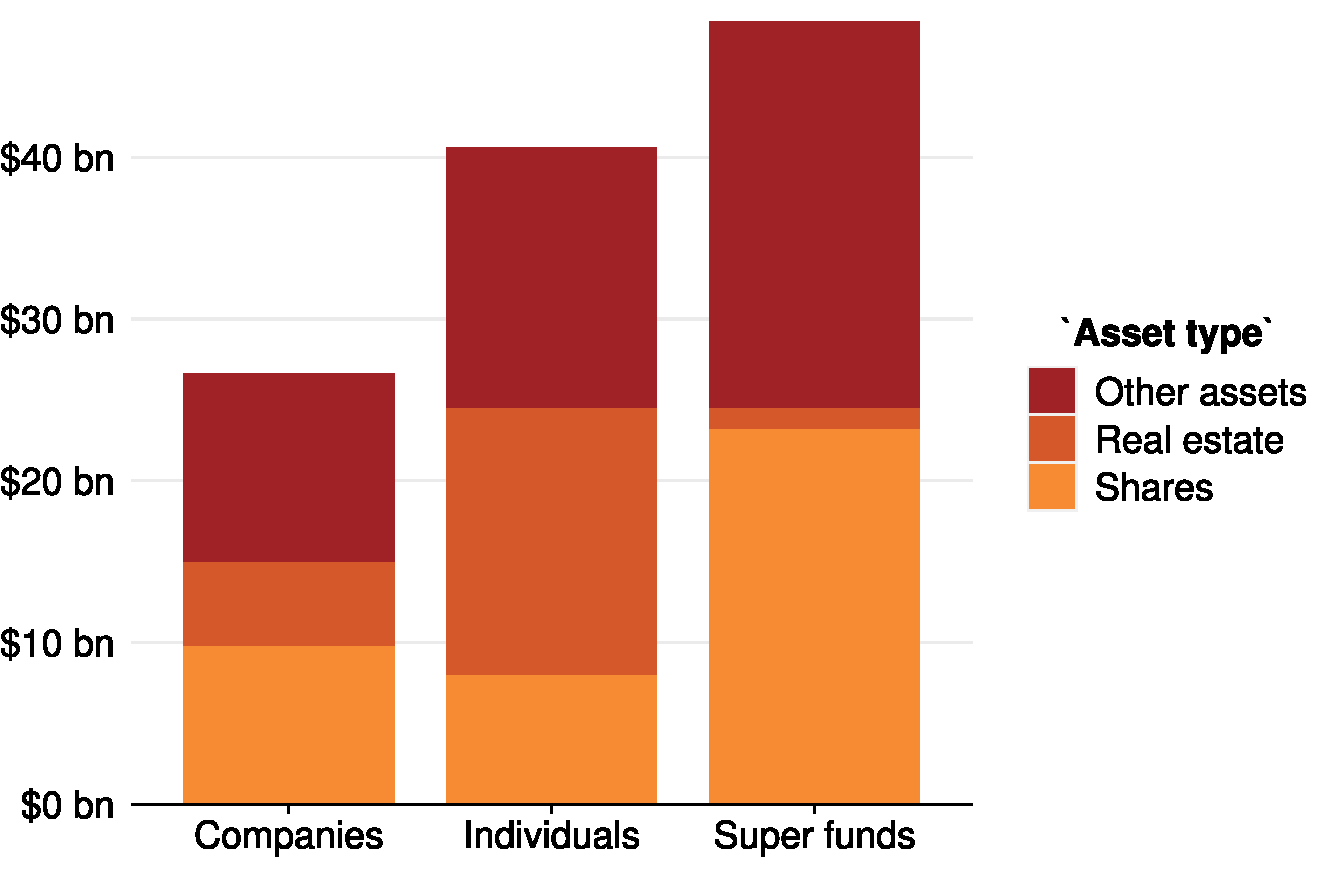
\includegraphics[width=\columnwidth]{CGT-NG-atlas//CGT-by-entity-asset-1}
\source{\url{http://data.gov.au/dataset/25e81c18-2083-4abe-81b6-0f530053c63f/resource/4e5cc0c1-a1b5-4bd2-80f4-6845ef78658b/download/Taxstats2014Summary5Index-of-chart-data.xlsx}}
\end{figure}

Capital gains are taxed as part of the income of individuals, companies and superannuation funds. In 2013-14, capital gains tax raised around \$7.5~billion, around 3\%\ of total income. This is expected to have climbed to \$8.9~billion in the following year.\footnote{2015-16 Budget Paper 1. Table 5 memoranda. \url{http://www.budget.gov.au/2015-16/content/bp1/html/bp1_bs4-03.htm}}

In 2018-19, capital gains tax was forecast to raise around \$16.6\,bn.%
  \footnote{MYEFO 2018-19; Note 3: Taxation revenue by type (continued). 
  \textcolor{blue}{\url{https://budget.gov.au/2018-19/content/myefo/download/MYEFO_2018-19.pdf}}.}


\section{Capital gains receive a range of tax advantages}
Before 1985, capital gains were not taxed in Australia. Since then, the tax treatment of capital gains has varied, but they have always been taxed at a lower rate than wage and salary income \Vref{box:Short-History}. 

\begin{smallbox}[!htb]{A short history of capital gains tax changes}{box:Short-History}
Before 1985 capital gains were untaxed in Australia. Taxes on capital gains were introduced to improve the integrity of the tax system, which was undermined by taxpayers recharacterising regular income as capital to avoid tax.   

Between 1985 and 1999, real capital gains (sale proceeds minus the original purchase price adjusted for inflation) were taxed at a taxpayer's marginal income tax rate. 

As recommended by the Ralph Review of Business Taxation, the Howard Government removed indexation adjustments so that tax was applied on nominal gains. To offset the removal of the indexation concession, capital gains tax was discounted by 50 per cent for individuals and 33 per cent for superannuation funds for assets held for more than a year. Capital gains of small unincorporated businesses, but not large businesses, are also discounted by 50 per cent. Small businesses also receive a range of other CGT concessions. When this regime was introduced, it was argued that it would stimulate capital markets and make the Australian regime more internationally competitive.
\end{smallbox}

For individuals and unincorporated small businesses, 50 per cent of their capital gains on assets held for more than one year are excluded from income. This means the effective tax rate paid on these gains is half the rate applied to other forms of income. Owner-occupied housing is an exception – capital gains on homes are not taxed at all. 

Superannuation funds pay tax on capital gains at 10 per cent (a discount to the 15 per cent they pay on earnings). 

Large corporations pay tax on their capital gains at the corporate rate of 30 per cent, which is the same rate as their income.

Capital gains also receive other less explicit tax advantages compared to recurrent income. First, capital gains are taxed on sale rather than as they accrue. This deferral of tax is akin to the government providing the investor with an interest free loan.  This substantially reduces the effective tax rate paid on gains, with the tax benefit increasing if the asset is held for longer.


With the 50 per cent discount, this deferral over 15 years for a top marginal rate taxpayer reduces the effective nominal tax rate on capital gains from 32 per cent to 28 per cent. (\Vref{fig:delaying-realization-causes-reduction-in-effective-tax-rate})

Second, investors are also able to choose the time of an asset's sale to minimise taxes on capital gains. They can reduce their tax by selling assets when their income is low, such as after retirement, so they are taxed at a lower marginal rate. Some Australians, particularly high income earners, wait until retirement to realise capital gains. Those 65 and older are much more likely to sell assets than those who are younger (\Vrefrange{fig:CGT-by-age-income}{fig:CGT-by-age-income-weight-CG}).



The benefits of waiting can be substantial. A person paying the top rate of income tax of 47\,c (including Medicare levy) who times the sale of an investment after 15 years for when they are in the lower tax bracket would reduce the annual nominal tax rate on that investment from 28 per cent to 26 per cent. The average marginal tax rate of those with capital gains tax was 30~percent; however, this weights an individual with a capital gain of \$1 equally as someone with a capital gain of \$500,000. Weighting by the value of capital gain, the average marginal tax rate was 42~percent. The average marginal tax rate on the first dollar of capital gains for people in the workforce is 29~percent compared to 20~percent for people over 65.








\begin{figure}
\Caption{Older taxpayers are more likely to have capital gains than younger taxpayers, for all age groups at almost all income levels}{Probability of net capital gains (2015-16)}{fig:CGT-by-age-income}
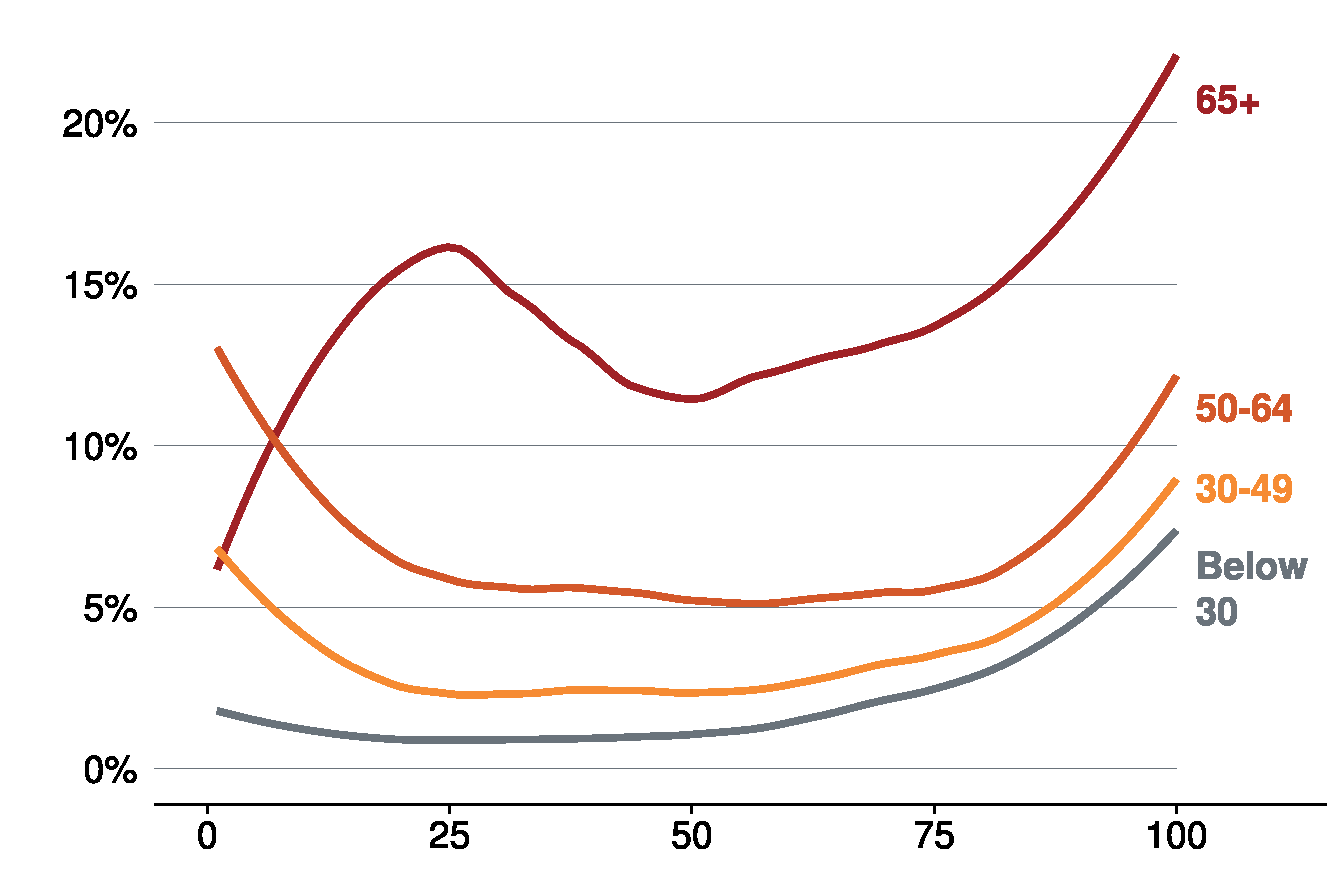
\includegraphics[width=\columnwidth]{CGT-NG-atlas//CGT-by-age-income-1}
\Caption{}{Average value of net capital gains}{fig:CGT-by-age-income-weight-CG}
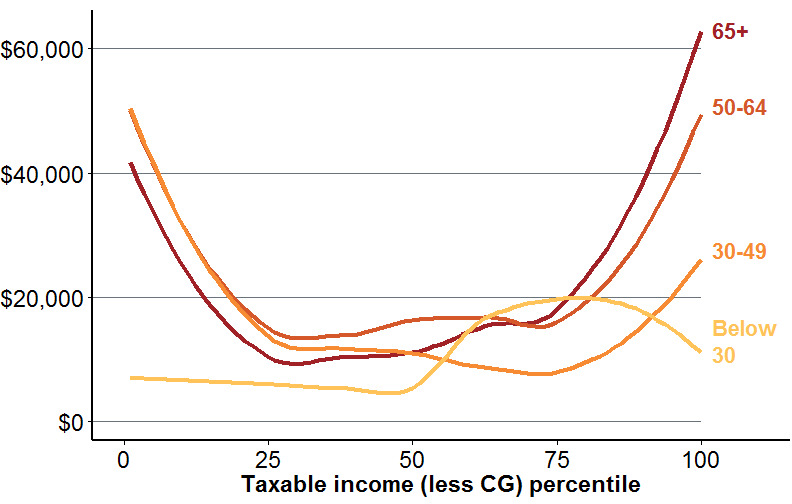
\includegraphics[width=\columnwidth]{CGT-NG-atlas//CGT-by-age-income-weight-CG-1}
\end{figure}






The benefits of waiting can be substantial. A person paying the top rate of income tax of 47\,c (including Medicare levy) who times the sale of an investment after 15 years for when they are in the lower (34.5\,c) tax bracket would reduce the annual nominal tax rate on that investment from 28~percent to 25~percent \Vref{fig:delaying-realization-causes-reduction-in-effective-tax-rate}.

\begin{figure}
\Caption{The delay in realizing capital gains subsantially reduces the effective tax rate}{Nominal effective marginal tax rates on savings}{fig:delaying-realization-causes-reduction-in-effective-tax-rate}
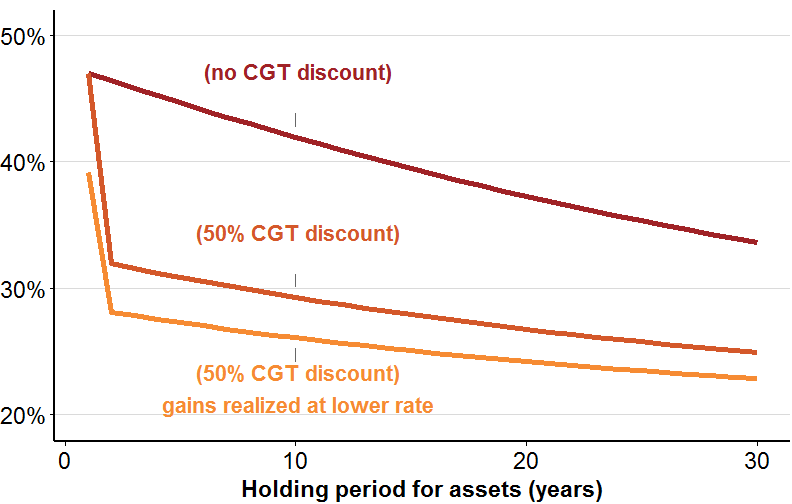
\includegraphics[width=\columnwidth]{CGT-NG-atlas//delaying-realization-causes-reduction-in-effective-tax-rate-1}
\end{figure}

\section{Adjusting for inflation}
In Australia, taxes on savings income, including capital gains, are levied on nominal returns, which include inflation. Because inflationary gains are not `income' in a true sense,  some discount on returns to savings is justified. But the 50 per cent discount has overcompensated property investors for inflation over time. 

A capital gains tax discount is an imperfect adjustment for inflation. The effective tax rate on real returns will depend on both the rate of inflation and the level of returns (Box x).  Under the 50 per cent discount, investors pay less tax compared to a tax on real gains so long as their asset values grow at least twice the rate of inflation. 






The 50 per cent discount has overcompensated property investors for inflation over the past 15 years. Since the introduction of the capital gains tax discount in 1999, house prices have grown annually by an average of 7~percent.  Inflation over this period averaged 3~percent annually. 

In contrast, long-term share investors who experienced low average capital returns because of the global financial crisis, would have been better off under a regime that taxed real capital gains. Share prices have grown by an average of only 3.6 per cent since 1999. 
 

\begin{smallbox}{The CGT discount has overcompensated property investors for the effects of inflation}{box:CGTOvercompensates}
The capital gains overcompensates many investors for the effects of inflation, especially when the other tax advantages for capital gains tax are taken into account.  

Under the 50 per cent discount, investors pay less tax compared to a tax on real gains so long as asset values grow at least twice the rate of inflation. The advantage is even larger on longer-term investments because capital gains tax is not paid until the asset is sold.

Since the introduction of the capital gains tax discount in 1999, house prices have grown annually by an average of 7.3 per cent  while share prices have grown by an average of only 3.6 per cent.  Inflation over this period averaged 2.8 per cent annually.  So the 50 per cent discount has overcompensated housing investors. In contrast, long-term share investors who experienced low average capital returns because of the global financial crisis, would have been better off under a regime that taxed real capital gains. Of course, both sets of investors received ongoing investment income in terms of rents and dividends that meant their net returns were significantly higher than those from capital gains alone.   
\end{smallbox}

\begin{smallbox}{Tax rates on real gains vary with inflation and returns}{box:tax-on-CG-vary-inflation-returns}
When taxes are levied on nominal returns then tax rates on real gains depend on both the inflation rate and the level of returns. 

% caching here might cause Sexpr to evaluate with reference to the wrong chunk.


Consider an investor Surya that has \$10,000 worth of shares. The shares pay no dividends so that all her returns are through capital growth.
Imagine the shares increase in value by 8~percent over the first year while inflation is 2~percent. If she sells the shares at the end of the year her nominal return is \$800. Her real (inflation-adjusted) return is \$540.\footnote{All printed numbers are rounded in this box.}

If she paid \highlight{tax directly on her real gain} at the 47\,c top marginal rate, she would pay \$252, and her \highlight{real after-tax return would be \$284.} If instead she paid \highlight{tax on her nominal gains with a 50 per cent discount} then she would pay tax of \$188 ($0.50 \times 0.47 \times \$800$) and she would receive a real after-tax return of \$349 (real return minus the \$190 tax). She is much better off\dots.



The opposite is true if her returns are low. To repeat myself, except with nominal rate of return set at 3~percent:

Consider an investor Surya that has \$10,000 worth of shares. The shares pay no dividends so that all her returns are through capital growth.
Imagine the shares increase in value by 3~percent over the first year while inflation is 2~percent. If she sells the shares at the end of the year her nominal return is \$300. Her real (inflation-adjusted) return is \$49.

If she paid \highlight{tax directly on her real gain} at the 47\,c top marginal rate, she would pay \$23, and her \highlight{real after-tax return would be \$26.} If instead she paid \highlight{tax on her nominal gains with a 50 per cent discount} then she would pay tax of \$70 ($0.50 \times 0.47 \times \$300$) and she would receive a real after-tax return of $-$\$22 (real return minus the \$70 tax).

\end{smallbox}





\section{Ideal tax rates on savings}
The ideal tax rate for the earnings on savings, and capital gains in particular, depends on competing considerations.
\newcounter{consideration}
\newcommand\consideration{\par\refstepcounter{consideration}\textbf{\textcolor{DarkOrange}{Consideration~\theconsideration:}}\hspace{2ex}}
\consideration Taxes on savings impose \highlight{costs}.
\begin{itemize}
  \item Taxes on savings discourage savings, instead encouraging immediate consumption
  \item Taxes on savings deter entrepreneurship by taxing the returns from taking a risk
\end{itemize}
\consideration The costs of taxes on savings must be balanced against the \highlight{costs of other taxes}. The relative size of the actual economic distortions matters.
\begin{itemize}
\item	Taxes on savings may not have much effect on actual savings and consumption choices. Behaviour both in Australia and overseas suggests that savers, particularly higher income savers are not very responsive to the tax rate in deciding how much to save.
\item	Capital gains taxes may not have much effect on entrepreneurship as a range of other tax breaks reduce the tax paid.
\item	Other taxes can impose significant economic costs. For example, income taxes (particularly on those earning between \$40,000 and \$80,000) can reduce incentives to work, particularly for those who require childcare if they work.
\end{itemize}
\consideration Differential treatment of some kinds of savings can distort investment choices, imposing other economic costs.
\begin{itemize}
\item	People tend to invest more in assets with high growth in their capital value rather than high annual income if the taxes on capital gains are lower than the taxes on income.
\end{itemize}
\consideration If earnings on savings are taxed less than wage income, the integrity of the income tax system may be undermined.
\begin{itemize}
\item 	Taxes on capital gains ensure that similar tax is paid whether receipts are classified as ``income'' or ``capital gain''; those on higher incomes tend to have more scope to structure transactions so that their earnings are classified as lower-taxed capital gains.
\end{itemize}
\consideration Lack of taxes on savings can reduce the progressivity of the income tax system.
\begin{itemize}
\item 	Taxes on savings limit the growth of inequality. People on relatively high incomes tend to save more; returns after tax greater than
inflation lead to them having even more to consume over their lifetime relative to those with low incomes.
\end{itemize}
All of considerations 2 to 5 above suggest that the tax rate on savings should be higher than if the theoretical ideal of consideration 1 is seen in isolation.

The remainder of this section works through these considerations in more detail.

\subsection{Not distorting decisions between consumption today and saving for tomorrow}
On the other hand, the theoretical ideal implicitly assumes losses and gains are taxed symmetrically. But this is not the case. Capital gains are taxed on realisation and at the time of the investors' choosing (section XX) whereas losses can be written off against taxable income each year. As we show in Chapter 4, this means that effective tax rates are lower for negatively geared investments than for investments fully financed from savings as is assumed in \Vref{fig:EMTR-savings}. Effective tax rates for investors under a range of alternative return scenarios and at different tax brackets are summarised in \Cref{appendix:EMTR}.





\begin{figure}[hb]
\Caption{The effective tax rate on excess returns for property has been close the income tax rate over the past 15 years}{Effective marginal tax rates on savings}{fig:EMTR-savings}


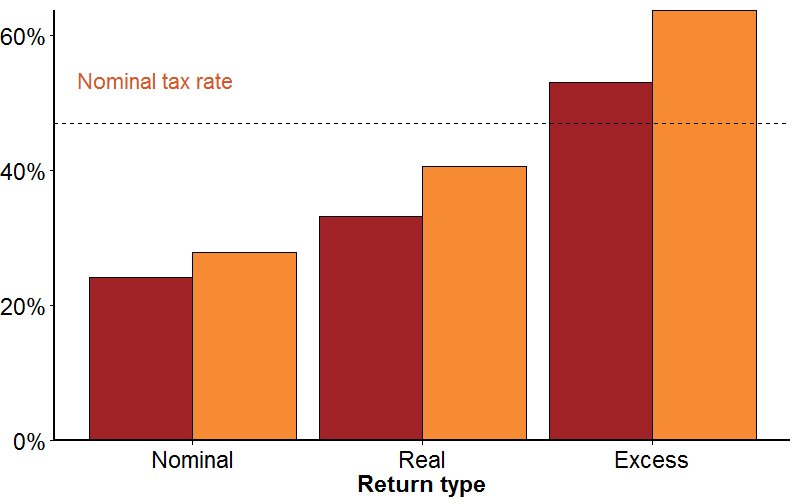
\includegraphics[width=\columnwidth]{CGT-NG-atlas//EMTR-nominal-real-excess-historic-vs-lower-1}
\end{figure}
\begin{table*}
\centering
\caption{Assumptions for \Vref{fig:EMTR-savings}}
\small
% latex table generated in R 3.5.2 by xtable 1.8-3 package
% Sun Jan 27 15:19:33 2019
\begin{tabularx}{\linewidth}{llrrrrrrr}
  \toprule
   &  &  &  &  & \multicolumn{4}{c}{\textbf{Constant}}\\
 \cmidrule(lr){6-9}
 \textbf{return type} & \textbf{scenario} & \textbf{capital gains} & \textbf{risk free rate} & \textbf{inflation} & \textbf{marginal tax rate} & \textbf{CGT discount} & \textbf{n} & \textbf{nominal rent}\\
 \midrule
excess & historic & 7.3\% & 5.6\% & 2.8\% & 47.0\% & 50.0\% & 15 & 3.0\% \\ 
   & lower & 5.0\% & 4.5\% & 2.5\% &  &  &  &  \\ 
  nominal & historic & 7.3\% & 5.6\% & 2.8\% &  &  &  &  \\ 
   & lower & 5.0\% & 4.5\% & 2.5\% &  &  &  &  \\ 
  real & historic & 7.3\% & 5.6\% & 2.8\% &  &  &  &  \\ 
   & lower & 5.0\% & 4.5\% & 2.5\% &  &  &  &  \\ 
   \bottomrule
\end{tabularx}

\end{table*}


\subsection{Maintaining the progressivity of the tax system}\label{sec:maintaining-progressivity-tax-system}


If returns to savings are not taxed, then inequality will tend to widen. The top ten per cent of wage and salary earners receive about 34~percent of all wages and salaries (before tax). They tend to save a greater proportion of their income than people who earn less, they are more likely to invest in higher risk, higher return assets, and they are more likely to make investments where a higher proportion of the returns are capital gains rather than income.  Consequently, among individual taxpayers, the top decile received 53~percent of all investment income, and 68~percent of all capital gains income (\Vref{fig:CG-by-decile} \&\ \Vref{fig:DecileStackedChart}). 

\begin{figure}
\Caption{Most capital gains are earned by those in the highest income decile}{Proportion of net capital gains by income decile (2015-16)}{fig:CG-by-decile}

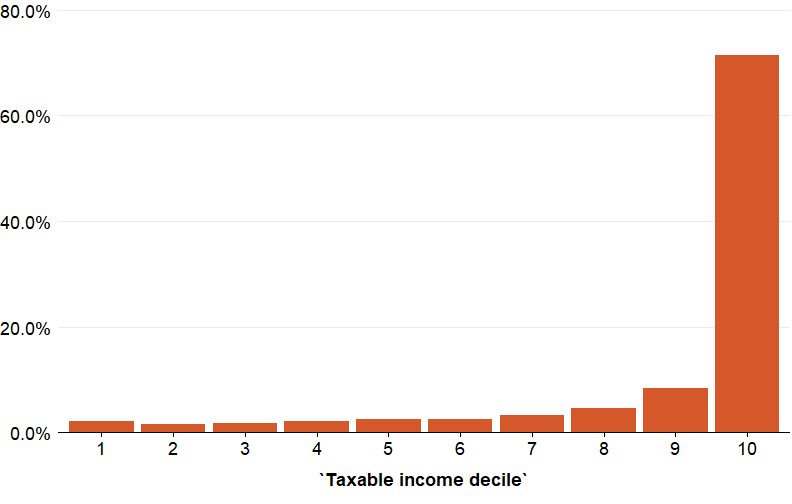
\includegraphics[width=\columnwidth]{CGT-NG-atlas//CG-by-decile-1}
\end{figure}



Because capital gains are lumpy, some lower income earners will have relatively high taxable incomes in the year they realise gains. But even if we look at taxable incomes \emph{before} capital gains, 30~percent of taxable gains are from the top decile. Another 26~percent are from those with less than \$10,000 in taxable income before capital gains.

Of the latter, many are over 50s that have waited until retirement to realise gains (section 2.2). There is also a sizeable group of 30-45 year olds with very high capital gains but no other taxable incomes (3~percent of taxpayers in this age group have capital gains in excess of \$10,000 and which make up more than 95\%\ of their total income).\marginpar{\textcolor{red}{\textbf{Not borne out.}}} Many are likely to be partners of high income earners that receive distributions of capital income through structures such as trusts. All of this is consistent with the finding that capital gains accrue disproportionately to those that are already well off. 

There is no reason a priori why any particular level of inequality is preferable to another, particularly if those levels of inequality are a consequence of some people working harder, or taking more risks, than others.  
However, if the returns on savings concentrate resources even more than wage inequality, then the reinvestment of the returns on savings can lead to continued increases in the concentration of wealth -- what Thomas Piketty described as an `endless inegalitarian spiral.'  Critics of Piketty's work, most notably Matthew Rognlie, argue that over the long-term, diminishing marginal returns should ultimately put a brake on the share of total income earnt by capital rather than labour.  However, Rognlie's finding that higher house prices (and associated economic rents) have been the dominant driver of the growth in the capital share of national income  do not undermine the Piketty thesis. Indeed, these findings suggest that so long as tight planning and zoning restrictions remain in place, those that can afford to save (and buy houses) are likely to keep capturing a growing share of national wealth.  

It is difficult to be comfortable with this outcome in which there is an ever-decreasing opportunity to save and garner substantial resources. This provides at least some justification for higher taxes on capital gains to break the cycle -- even taxes on the inflationary component of capital gains which act as de facto wealth taxes.  

Another version of this argument is that tax concessions for capital gains make Australia's income tax system less progressive than is implied by income tax rates. While some may want a less progressive system, tax concessions are generally a poor way to achieve this, because they are inherently less transparent than changing the marginal rates of income tax. For value choices such as the progressivity of the tax system, the public debate is best served by making the distribution of the tax burden as transparent as possible.

\subsection{Distortion of investment choices}
Providing a tax discount for capital gains but not for other investment income distorts investment choices. 

Capital gains have substantial tax advantages relative to annual earnings. The capital gains discount magnifies the tax advantages because capital gains are not taxed until they are realised (Figure 2). In contrast, Australia's current tax system does not adjust for the effects of inflation on bank deposits, which are assets disproportionately held by the least well off.  Rental income, bond yields and returns from overseas shares are also taxed at full marginal rates.

Taxing capital gains more lightly than most other savings income creates an incentive for investors to choose riskier assets that return more via capital gain. In conjunction with generous rules for deductibility of interest costs, the tax system creates strong incentives for debt-financed and speculative investments (section 3.1). As a result, Australians invest more in property and less in bank deposits than economic fundamentals would suggest is ideal.

The efficiency losses generated by the different tax treatment of different forms of savings are likely to be much larger than from the weight of taxes on capital in general.   Of course, the economic cost of differing tax treatments is also an argument for taxing savings earnings less rather than taxing capital gains more. But substantial budget deficits leave little room to reduce taxes on other forms of savings income. Consequently, the most plausible way in practice to reduce the distortions between different forms of savings is to increase the taxes on capital gains (section 4.4). 

However, increasing taxes on capital gains will increase the incentives to invest in owner-occupied properties and in superannuation, which already enjoy even larger tax concessions than capital gains. People would be encouraged to invest even more in their principal residence, by renovating, and purchasing bigger and better-located homes. 

There is some truth to these concerns, but they shouldn't be overstated. 

First, there is at least a plausible rationale for encouraging additional investment in owner-occupied housing,  the biggest single component of wealth.  Governments have deliberately promoted home ownership because of the social benefits including enforced savings, social stability and community involvement.  Therefore, further widening the tax advantage for owner occupied housing by reducing the CGT discount may not be a net social cost. 

While some tax incentives for superannuation might be justified, the current regime is too generous and poorly targeted. Grattan Institute's 2015 report, \textit{Super tax targeting}, argues that they should be wound back.  In the meantime, failure to reform superannuation should not hold back capital gains tax reform. 



Second, reducing the discount might not lead to much greater investment in owner-occupied housing and superannuation. Households already hold 42~percent of their assets outside these areas, even though they have substantial tax advantages. This is presumably because people want savings in forms that are available for use before retirement and without having to sell their home.  





\begin{figure*}
\Caption{}{Distribution of taxes and income by taxable income decile}{fig:DecileStackedChart}
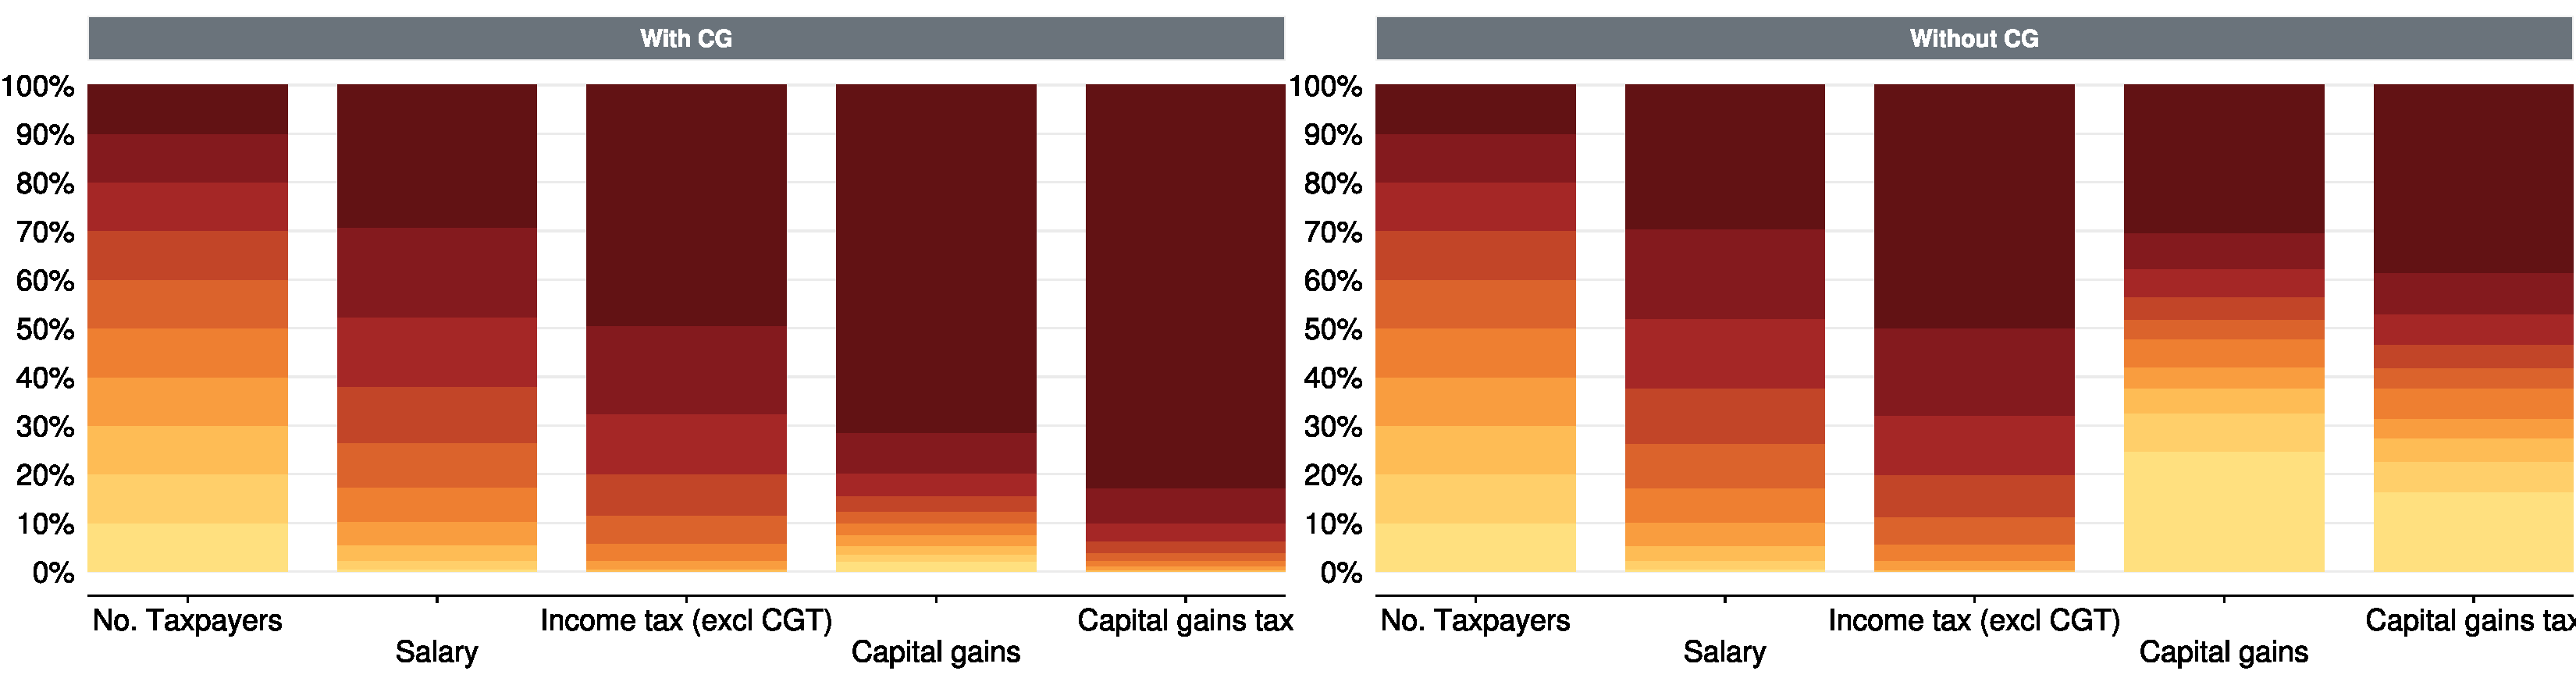
\includegraphics[width = \textwidth]{CGT-NG-atlas//stacked-column-chart-1}
\the\textwidth
\end{figure*}

\chapter{Negative gearing}
Negative gearing allows taxpayers to subtract the losses they make on
investments (after costs including mortgage interest payments) from
their taxable income including wages.

The ability to deduct expenses incurred in generating assessable income
is part of the normal operation of the Australian tax system, and
applies to a wide range of investments and business activities. If
losses were not deductible, they would be treated asymmetrically to
gains (which are taxed) and investments in risky assets would be less
attractive. Deductibility of interest payments in theory maintains tax
neutrality for investors choosing between debt and equity
financing.\footnote{Fane and Richardson (2004)}

But there is no theoretical basis for allowing losses on investment to
be deducted against entirely unrelated income such as wages. Indeed,
allowing full deductibility of investment losses against wages when
capital gains are taxed concessionally and only on realisation leads
investors to favour debt financed investments that generate more of
their returns via capital gains in order to maximise tax breaks on
wages. This reduces tax collections and has negative impacts in
investment markets, particularly housing markets, where the tax
treatment has encouraged speculative activity.

Most other advanced economies provide a less generous treatment for
rental losses. The United States only allows losses to be written off
against other forms of ``passive'' income.\footnote{Passive income is
  defined as income from rental properties or businesses in which the
  taxpayer does not materially participate. It is distinct from active
  income (wage, salary and income from business in which the person is
  actively involved) and portfolio income (income from interest,
  dividends etc). See: IRS (2015).} The UK and many European countries
only allow deductions against the same \emph{class} of income, so for
example, losses on investment property can only be used to reduce tax on
income or capital gains from other investment properties. Others such as
the Netherlands do not allow deductibility of losses from investment
housing (Appendix C).\footnote{Summaries of international regimes can be
  found in RBA (2014), p. 43; Productivity Commission (2004), p. 86;
  O'Donnell (2005), pp. 92-95.}

\section{Negative gearing provides a tax shelter against
wages}\label{negative-gearing-provides-a-widely-used-tax-shelter-on-wages}

Negative gearing allows taxpayers to subtract the losses they make on investments from their taxable income including wages. Losses are defined as investment expenses in excess of rental income.  Expenses include interest on borrowing to purchase the asset, which are about half of the costs of property investors.  

Taxes on capital gains are discounted by 50 per cent and only paid when
the asset is sold. But negative gearing arrangements allow investors to
deduct losses -- investment expenses (including interest costs) in
excess of rental income from wage income that would otherwise be taxed
at the full marginal rate.\footnote{In reality, the assets are generally
  not making a loss because they are accruing a capital gain. But these
  gains are not included in the definition of taxable income from the
  asset until they are realised. See: ACOSS (2015), pp.12-13.}

With the right investment strategy, an investor can use this asymmetry
in the tax treatment of gains and losses to pay less tax in total and
later despite receiving additional investment income (\Vref{box:NG-to-reduce-tax-on-wages}).

\begin{smallbox}{Using negative gearing to reduce taxes on wage income}{box:NG-to-reduce-tax-on-wages}
High income investors can maximise the tax shelter on their wage income
by borrowing to invest in assets that generate less in recurrent income
and more through capital gains.



Suppose Dan, a lawyer earning \$250,000 a year, 
borrows \$750,000 %
(interest only)
to purchase a \$750,000 investment property. Interest on the loan is 6~percent a
year and the property generates a rental return of 2~percent each
year. Most of the property's return is via capital appreciation of 5~percent each year.

In the first year, Dan makes a loss of \$26,000 
on the property and
reduces the tax he pays on his \$250,000 salary by 
\$13,000. His rental
losses decline over time as the property appreciates. After five years,
Dan has reduced taxes on his wage income by a total of 
\$70,000. If he
sells the property after five years he will realise a capital gain of
\$210,000 and pay tax on 
the gain of just under \$51,000.

Because of the asymmetry of tax treatment of gains and losses, Dan pays
\$8,700 less tax in total over five years than if he had not purchased
the house. So despite his profit of more than \$86,000 on the
investment, he has reduced his tax considerably.
\end{smallbox}
Tax deductions from wage income may also generate ``psychic payoff'' for
some investors -- the pleasure of denying the Tax Office its due. As an
investment strategy, negative gearing only makes sense if the expected
capital gains exceed the rental losses over the life of the
investment.\footnote{And this is more than the returns that could have
  been generated through other investments.} But for some investors,
reducing taxes on their wages has become one of the primary goals.
Investment advisors have warned against investors placing too much
emphasis on tax breaks and not enough on the financial returns to the
investment.\footnote{See for example: Brown (2012). There is some
  evidence from the US of taxpayers placing disproportionate weight on
  tax deductions for investments . For example, taxpayers are far more
  likely to contribute to a tax deductible retirement saving account if
  they owe money to the Internal Revenue Service in excess of taxes
  withheld. Hubbard and Skinner (1996), p.76.}
  


\begin{figure}[!htb]
\Caption{More people negatively gear property investments in their peak earning years}{Percentage of 2015-16 taxpayers with }{fig:NG-PG-by-age}

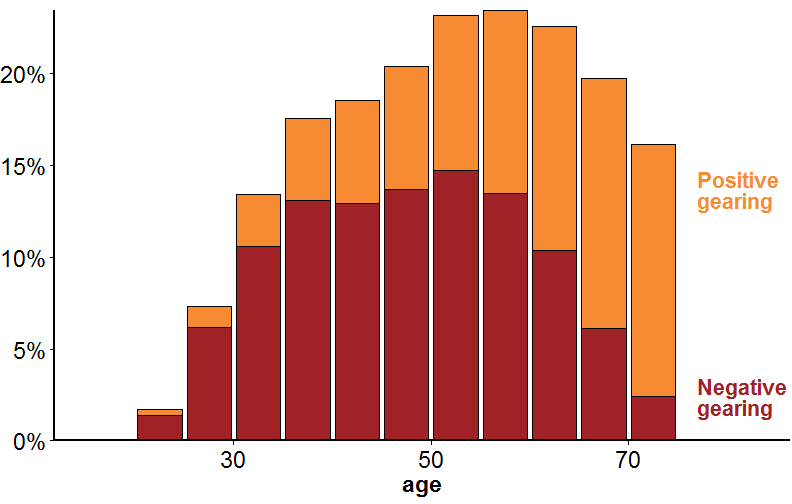
\includegraphics[width=1.225\columnwidth]{CGT-NG-atlas//NG-PG-by-age-1}
\source{2015-16 sample file.}

\notes{Taxpayers over the age of 70 are not disaggregated in taxstats and have been presented as having ages 70-75.}
\end{figure}

The attractiveness of using investment losses to reduce taxes on wage
income is evident in the age profile of those negatively gearing
property. Investing in loss making properties is popular amongst those
of working age, but far less prevalent amongst over 60s who are unlikely
to benefit from the tax write-offs. 68~percent of those under 60
with investment properties make rental losses compared to less than 33~percent over 60 (see \Vref{fig:NG-PG-by-age}).

Of course, not all investments are negatively geared. `Positively geared' properties are those where the annual income on the property exceeds the annual costs of maintenance and interest. Typically, positively-geared investors have broowed less of the value of the property, and so they have lower interest costs.

Negative gearing is used much less for investments outside of housing. Investors in assets other than real estate, such as equities or unincorporated businesses, are less likely to borrow some of the funding, and usually do not borrow so much that these investments are negatively geared. 

Total lending to individuals for share investments is at most \$19 billion, compared to individuals' direct share holdings of around \$550~billion,\footnote{The ATO reported that the 2013-14 dividend income for individuals was \$23.8~billion. The HILDA survey showed in the same year \$0.969~trillion for household wealth in equities.}  and compared to borrowings of \$548~billion from banks for housing investor lending. 

When individuals do borrow to invest in equities, they are seldom negatively geared. Equities investors will only be negatively geared if they are at least 70 per cent leveraged.  The average leverage of those who do have a margin loan is around 27 per cent.  Few margin lending investors leverage more than 65 per cent. Usually the maximum leverage permitted is around 75 per cent. Most margin lending customers dislike margin calls, and so they tend to create a buffer of at least 10 per cent less than this. 





Very few loans to invest in unincorporated businesses will be negatively geared. Banks are understandably reluctant to lend to businesses that do not have enough cashflow to cover interest payments. Total interest costs for unincorporated businesses were \$1.34~billion in 2015-16  (much smaller than negative gearing against property), and much of this would have been incurred by profitable businesses. And unincorporated business losses totalled \$4.32~billion \TBD{(section 5.2.3)}; many of these businesses would not have borrowed. 

\section{Negative gearing goes beyond generally accepted principles for offsetting losses against gains}
The ability to deduct expenses incurred in generating assessable income is part of the normal operation of the Australian tax system, and applies to a wide range of investments and business activities. If losses were not deductible but gains were taxed, the asymmetry would make high-risk (high expected return) assets a less attractive investment. Deductibility of interest payments in theory also maintains tax neutrality for investors choosing between debt and equity financing.  

But there is no theoretical basis for deducting losses on investments from entirely unrelated income such as wages. This is reflected in provisions that limit the deduction of business losses from wage and salary income. 

Some other advanced economies restrict the deduction of rental losses from wage and salary income. The United States only allows losses to be written off against other forms of ``passive'' income.  The UK only allows deductions against the same class of income, so for example, losses on investment property can only be used to reduce tax on income or capital gains from other investment properties. Others such as the Netherlands do not allow deductibility of losses from investment housing (Appendix C). 

Indeed, the Commonwealth Government already implicitly accepts the principle that investment losses should not always be applied in calculating tax and welfare outcomes. Ironically, these restrictions currently only apply to those on lower incomes. Calculations of income support payments do not allow people to reduce their taxable income through investment losses. Income tests for Family Tax Benefit Part~A and Part~B, Child Care Benefit are based on `adjusted taxable income', which adds back investment losses. 

\section{The tax advantages of negative gearing distory investment choices}
Investment choices are severely distorted when negative gearing is permitted and capital gains are taxed concessionally and only when realised. This regime encourages investors to leverage more, to favour investments that return capital gains rather than income, and to churn their investments more often.

\subsection{Bias towards higher leverage}
The asymmetry between the tax treatment of gains and losses makes debt financing of investment more attractive. For a high income taxpayer investing in a rental property, real effective marginal tax rates are substantially lower for a property financed through borrowing. The higher the gearing, the lower the effective marginal tax rate (\Vref{fig:EMTR-by-gearing}). 

\begin{figure}
\Caption{Effective tax rates depend on amount of borrowing}{Real effective marginal tax rate}{fig:EMTR-by-gearing}

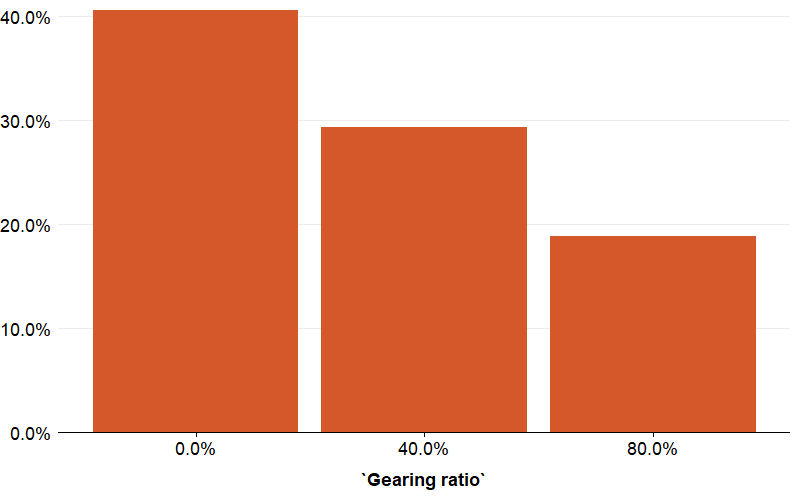
\includegraphics[width=\columnwidth]{CGT-NG-atlas//EMTR-by-gearing-1}
\source{Grattan analysis}

\notes{Assumes 
3~percent nominal rent income, 
5~percent capital gain per year, 
2~percent inflation,
5~percent interest rate on borrowing, 
50~percent CGT discount, 
and
47~percent marginal tax rate. 
The property is held for 
15 years and then sold.
}
\end{figure}

The Henry Tax Review described the asymmetry between gains and losses as ``among the greatest tax induced biases to the savings choices of households''.  This contradicts the rationale for allowing the deductibility of losses -- to maintain tax neutrality of debt and equity financing.

Indeed, the distortions created are so large that it is possible that an investment with a negative pre-tax return over its lifetime can nevertheless provide a positive return to its investor after taking into account the tax benefits.  

While this bias towards higher leverage applies to all investments, in practice, it encourages greater investment in property because bank lending rules allow greater leverage than for others assets such as shares.

\subsection{Bias towards capital gains not annual returns}
As the RBA notes:

\begin{quote}
\dots\ in most countries the earning of rental income is seen as the most important reason for investing in rental properties\dots{}. This seems to stand in contrast to the situation in Australia where properties are commonly marketed on the presumption that they do not earn positive taxable income for a considerable period.
\end{quote}

\textcite{SeeligThompsonBurkeEtAl2009} echoes the RBA view, finding that the majority of property investors saw capital gains as more important that rental income in motivating them to invest in property.


These biases are not just theoretical arguments. They are reflected in how investors have changed their behaviour since capital gains tax changes increased the attractiveness of negative gearing from 1999.




\begin{figure}
\Caption{More people are negatively gearing and have higher losses}{Number of people negatively gearing property 1993-94 to 2015-16}{fig:number-NG-time-series} 
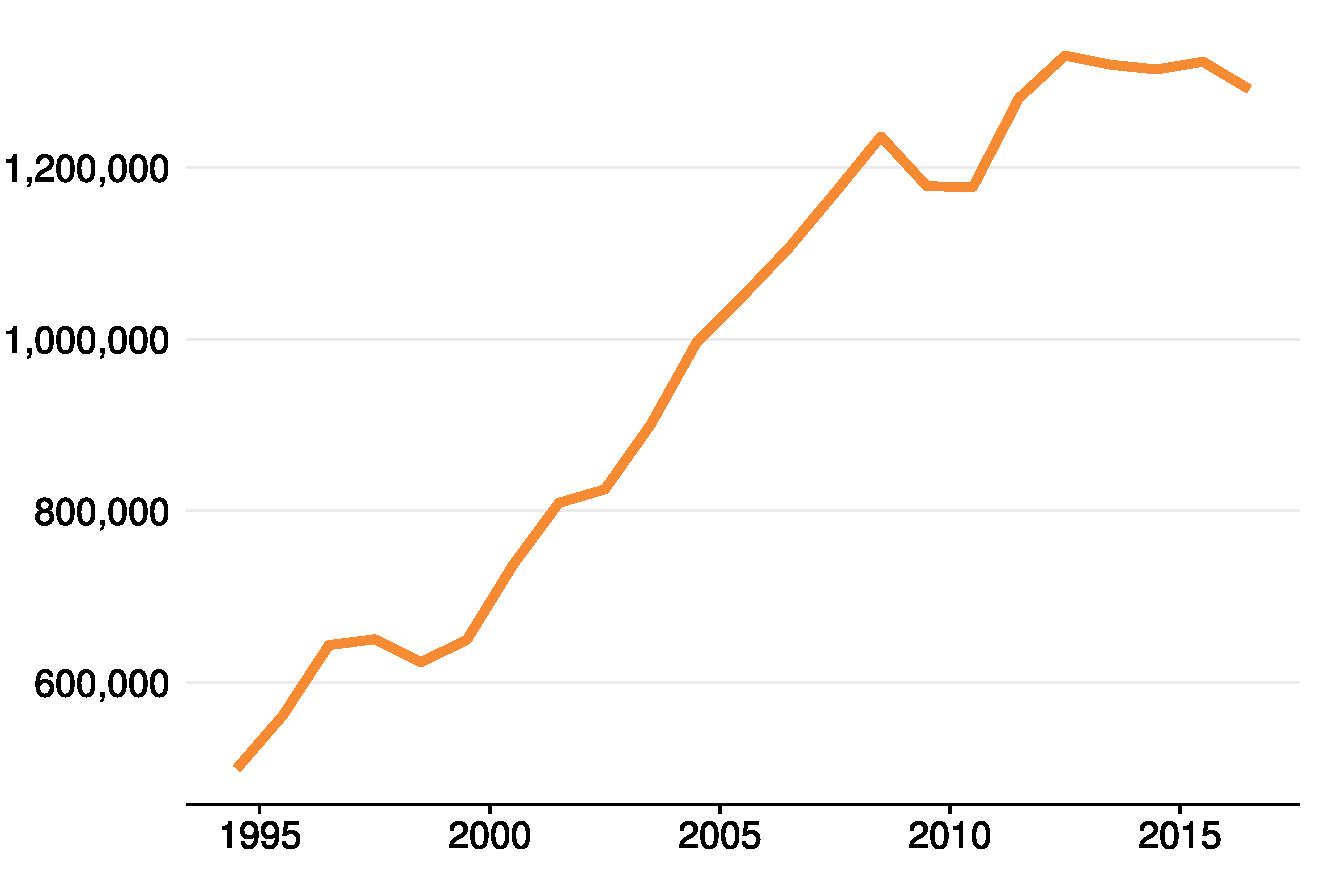
\includegraphics[width=\columnwidth]{CGT-NG-atlas//number-NG-time-series-1}
\vspace*{4pt}
\captionsetup{font = {small, color=theGrey}}
\caption*{Average net rental loss, (2017-18 dollars)}\label{fig:number-NG-and-net-losses-time-series}
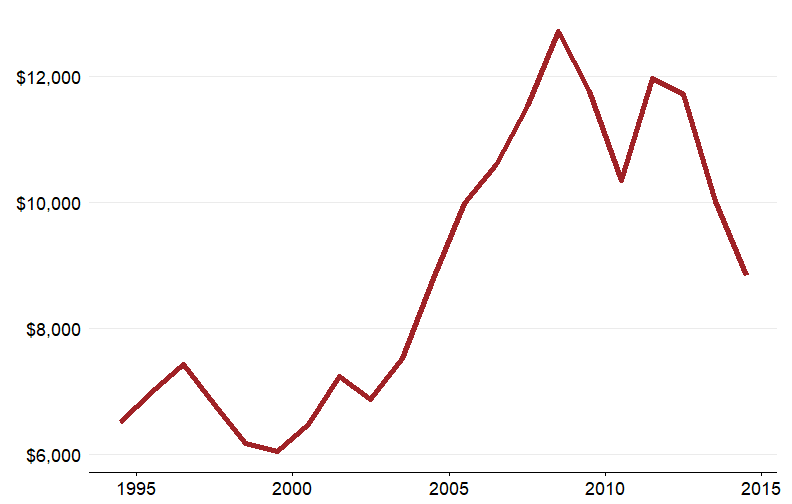
\includegraphics[width=\columnwidth]{CGT-NG-atlas//avg-net-losses-time-series-1}
\end{figure}

Negatively geared residential property investments have grown rapidly over 20 years, particularly after 1999 when the capital gains discount changed from taxing all real gains to taxing half of the nominal gains. Over 15 years the number of taxpayers making losses on residential property has almost doubled, as has the size of the average loss in real terms (\Vref{fig:number-NG-time-series}).

\begin{figure}
\Caption{Almost all the growth in property investment since 1994 has been because of loss-making landlords}%
{Number of landlords with positive and negative net rental income, 1993-94 to 2015-16}{fig:number-of-investors-by-gearing}

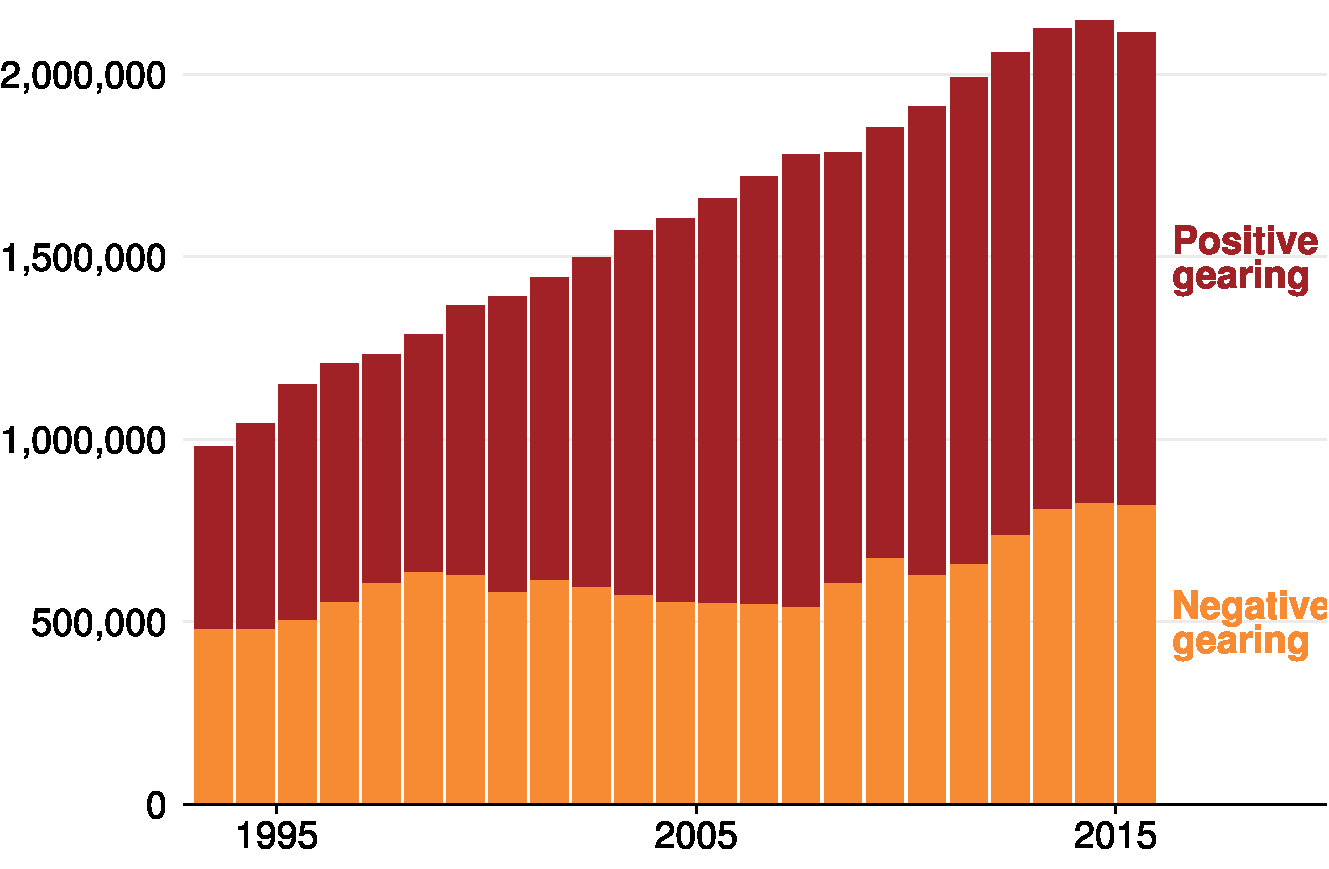
\includegraphics[width=\columnwidth]{CGT-NG-atlas//number-of-investors-by-gearing-1}
\end{figure}

\textcite{SeeligThompsonBurkeEtAl2009} find that around half of investors would not have invested in property if negative gearing had not been available.  Meanwhile there has been little change in the number of positively geared investors. Almost all the additional investors in property over the last 15 years were negatively geared (\Vref{fig:number-of-investors-by-gearing}).


 
 And the average level of gearing for property investors is increasing.
 Even though interest rates are falling, interest deductions as a proportion of rents increased from 45.6~per cent of gross rental payments in \mbox{1997-98} to 84.2 in 2007-08. With falling interest rates, interest deductions as a proportion of gross rents had fallen to 51.6~per cent in 2015-16.
 


As a result, Australian landlords have moved from being collectively profitable, to accruing billions in net rental losses each year. In 2015-16, 1.29~million landlords reported collective losses of \$11.3~billion. Consequently, total net rents have been consistently negative since the introduction of the CGT discount. (\Vref{fig:Net-rent-time-series}).  Losses are reducing only because interest rates have fallen rapidly.

\begin{figure}
\Caption{Since the introduction of the capital gain tax discount, rental losses have been large, overwhelming profits}{Total real net rent (profit \(-\) loss), individual taxpayers, (2017-18 dollars)}{fig:Net-rent-time-series}

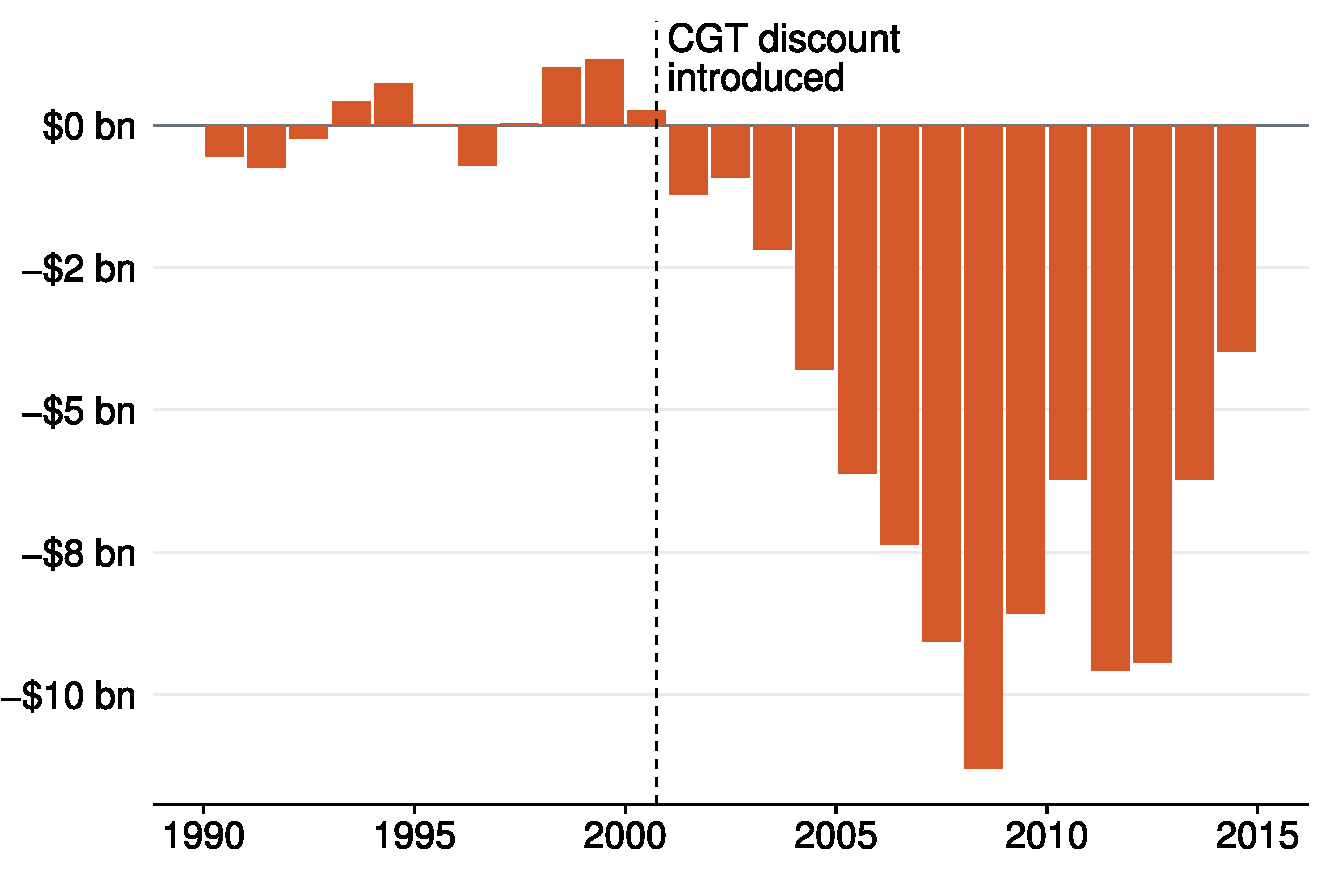
\includegraphics[width=\columnwidth]{CGT-NG-atlas//Net-rent-time-series-1}
\end{figure}

\subsection{Property churn}
The tax advantages encourage those with negatively geared properties to ``churn'' investments. Properties do not stay negatively geared. Rents tend to rise over time with increases in the value of wages, whereas the tax deductible loan value cannot be increased.  So if an investor wants to stay negatively geared, they need to sell, and then purchase another property with borrowings that are again a large proportion of the investment.

Consequently, negatively geared investors turn over their investments more often. \textcite{Wood2010a} showed that 40 per cent of all investors with rental properties retained their property at the end of a 5 year period.  Amongst investors that were negatively geared, however, only 20 per cent retained ownership. And a greater proportion of negatively geared landlords than other landlords purchased another property after selling.  

\section{The distortions caused by negative gearing have undesirable social consequences}
Negative gearing has many undesirable social consequences. It reduces rates of home ownership. It reduces the availability of long-term rentals. It increases the volatility of housing markets, increasing the risks of the Australian financial system. 

The favourable tax treatment reduces home ownership because it increases the after-tax returns to geared property investors but not homeowners. The increase in geared investing has crowded out purchases by owner-occupiers. Investors now account for more than 50 per cent of new loans for housing, up from 29 per cent two decades ago.  This is one of the reasons (but by no means the only reason) that rates of home ownership are falling among younger age groups.

The higher churn of properties encouraged by negative gearing also contributes to the lack of secure long-term tenancies in Australia. Most of Australia's housing stock is owned by landlords with only one or two properties, because progressive land taxes significantly reduce the returns from larger landholdings.  As many of these landlords are negatively geared, and want to turn over their properties in order to stay negatively geared, most Australian landlords are reluctant to agree to long-term tenancies. Their political interests have also led to Australian tenancy law providing much less security for tenants than in other countries. 

Negative gearing contributes to volatility in housing markets, as suggested by the Reserve Bank, the Productivity Commission, the Henry Tax Review, and the Murray System Inquiry.  Negative gearing is most attractive as a tax minimisation strategy when asset prices are rising strongly. So in boom times it further increases investor demand for housing. The opposite is true when prices are stable or falling. Consequently, the greater leverage encouraged by negative gearing arrangements also reduces the stability of the Australian financial system.

There is little evidence that negative gearing has the socially desirable outcome of reducing rents, as discussed in \Vref{sec:taxes-not-change-rents-much}.

\section{Negative gearing mainly benefits those on higher incomes}
Like most tax concessions on investment, tax benefits from negative gearing are regressive, benefiting those on high incomes much more than those on low incomes. A higher proportion of taxpayers on higher incomes negatively gear and the tax break is usually larger for individuals on higher marginal tax rates. 

The fact that negative gearing is regressive is not in itself an argument for change, as discussed above in \Vref{sec:maintaining-progressivity-tax-system}. However, as that section argues, lower taxes on savings can concentrate wealth, and the inherent lack of transparency of tax concessions can undermine the overt choices in income tax scales about the desired level of redistribution. So it is important to understand how the benefits of negative gearing are distributed. This analysis is also relevant to counter claims that negative gearing should be retained because it particularly assists those on middle incomes to build wealth. 



A lot of the public debate has centred on claims that most taxpayers negatively gearing have taxable incomes below \$80,000. This is not surprising given that only 21~percent of taxpayers have higher taxable incomes. 

\begin{figure}
\Caption{More taxpayers on higher incomes negatively gear}{Distribution of taxable incomes by negative gearing status, 2013-14}{fig:tx-inc-distr-by-NG}
% dev omit emf due to alpha


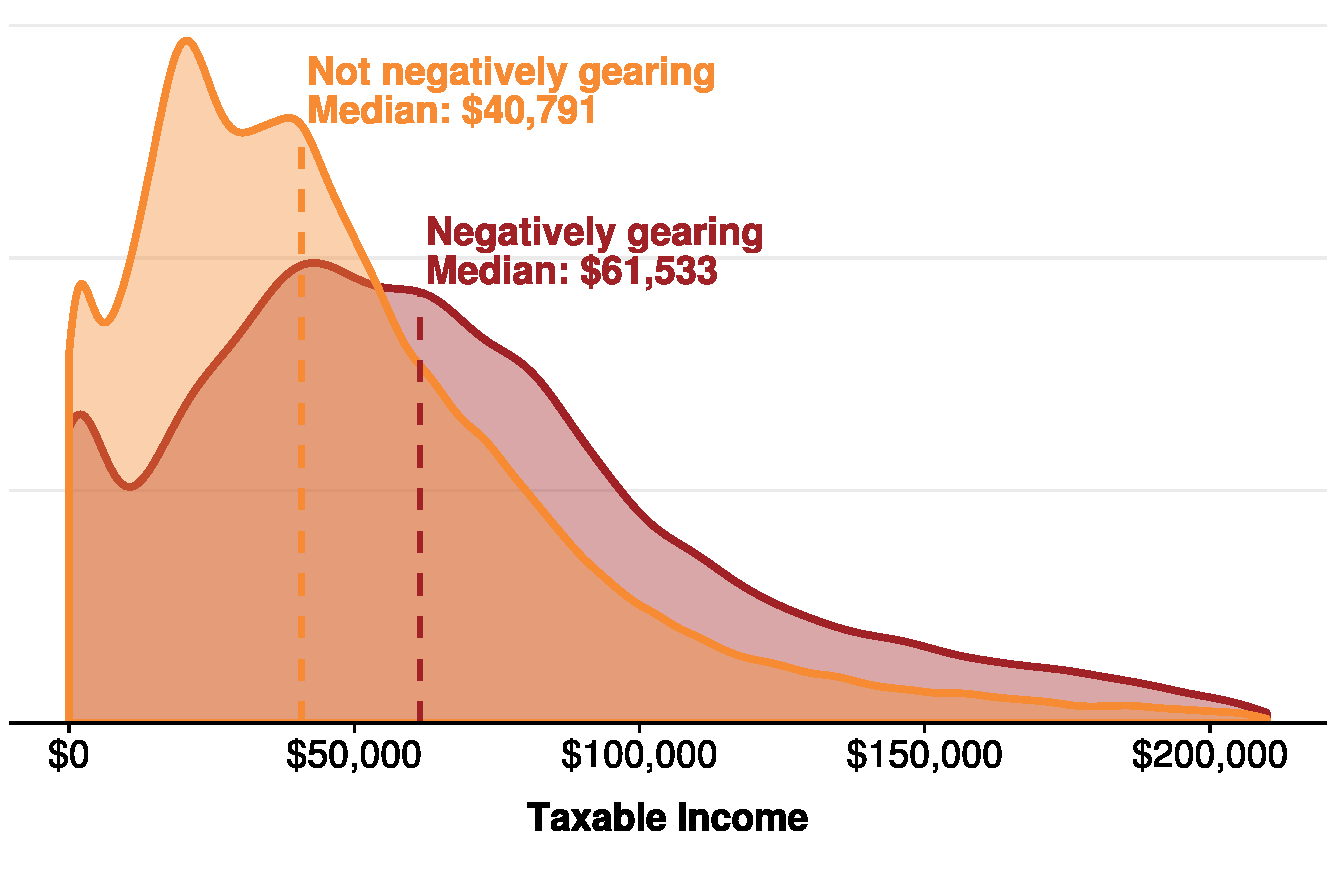
\includegraphics[width=\columnwidth]{CGT-NG-atlas//tx-inc-distr-by-NG-1}
\end{figure}

\begin{figure}
\Caption{More taxpayers on higher incomes negatively gear (2015-16)}{Distribution of taxable incomes by negative gearing status, 2015-16}{fig:tx-inc-distr-by-NG-latest}
% dev omit emf due to alpha

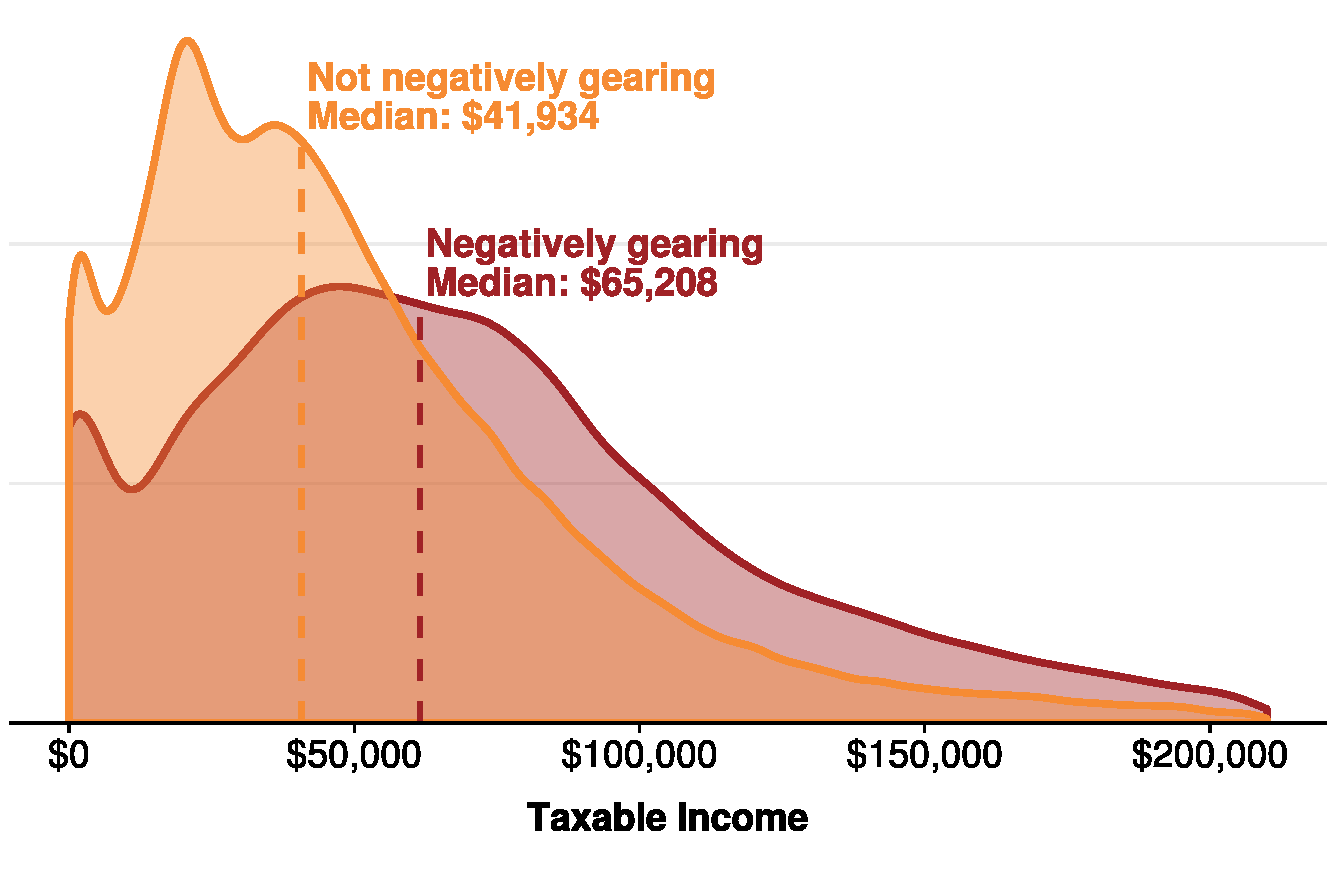
\includegraphics[width=\columnwidth]{CGT-NG-atlas//tx-inc-distr-by-NG-latest-1}
\end{figure}


As shown in \Vref{fig:tx-inc-distr-by-NG}, people with higher incomes are more likely to negatively gear. The median taxable incomes for taxpayers that negatively gear is \$65,000 compared to  \$42,000 for those taxpayers that don't negatively gear.


The tax benefits from negative gearing are even more skewed toward high income earners. They are more likely to borrow more, and with higher marginal tax rates, the deductions are worth more. 





\begin{figure}
\Caption{Negative gearing mostly benefits those on high incomes, and the difference is especially stark when incomes are measured before subtracting rental interest deductions}{Percentage of each decile's share of the benefit in reduced income tax due to negative gearing (2015-16)}{fig:Benefit-NG-before-after-deductions}
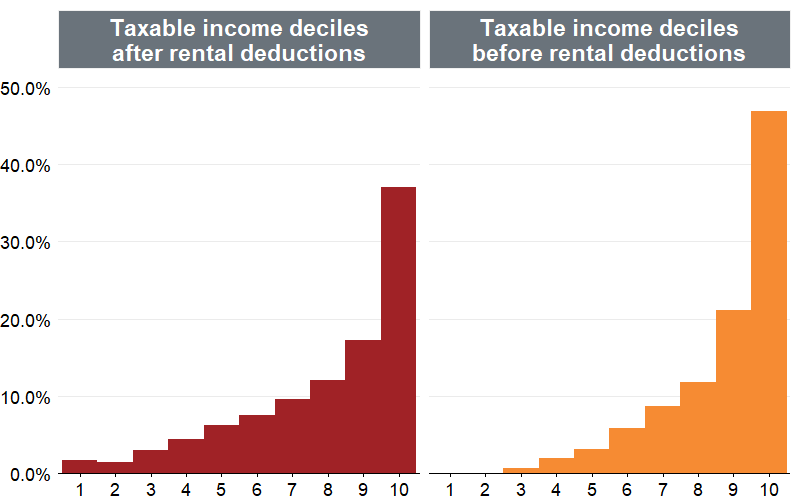
\includegraphics[width=\columnwidth]{CGT-NG-atlas//Benefit-NG-before-after-deductions-1}
\notes{Taxable income before rental deductions means \(\text{Taxable Income} - \min(\text{Net rental profit}, 0)\).
Income tax includes medicare levy, LITO, and the temporary budget repair levy but not other tax benefits (\emph{e.g.}~the seniors and pensioners tax offset (SAPTO))}

\source{\gao\ 2015-16 sample file}
\end{figure}

Overall, the top ten per cent of income earners before rental deductions receive over~47~percent 
of the tax benefits of negative gearing. The skew does not look quite so bad if taxpayers are grouped by their taxable incomes, as shown in the left hand side of \Vref{fig:Benefit-NG-before-after-deductions}. But comparisons based on taxable incomes understate the earnings of those that are negative gearing. Taxable incomes are assessed after rental losses. In other words, people who are negatively gearing have lower taxable incomes because they are negatively gearing. The distribution before rental deductions, shown on the right hand side of \Vref{fig:Benefit-NG-before-after-deductions}, shows that those on higher incomes receive the lion's share of the tax benefits from negative gearing.

%\flushcolsend
\chapter{Impact of changing negative gearing and the CGT discount}
Much of the political debate surrounding changes to negative gearing and the CGT discount have centred around the impact on investor demand, rents and property prices. 

Limiting loss write offs and increasing the effective tax rate on capital gains will reduce the after-tax returns on property investment. This will somewhat reduce investment demand. 

Economic theory suggests that the impact will be some combination of higher rents and lower house prices. But in urban housing markets with tight constraints on supply and where locational factors strongly influence rental demand, almost all of the impact will be on prices.  

But the price impacts will not be large. Our proposed reduction in tax concessions will result in modest changes in effective tax rates for investors. And owner occupiers -- the majority of property buyers -- face no change in their after tax returns. Our best estimate is that property taxes changes might reduce house prices by up to a one-off \TBD{xx -xx\%}, depending on how much the capital gains tax discount is reduced. There will be very little impact on rents, even after a decade.

\section{Tax changes will somewhat reduce investor demand}
Reducing the capital gains tax discount and limiting scope for loss write offs by changing negative gearing arrangements will somewhat increase the effective tax rates for property investors. 

Some investors will switch to other investment opportunities that offer higher post-tax returns. Others might choose to spend more and invest less. But some will also continue to invest in the housing market, and either borrow less, or simply accept a lower return on investment.

But the extent to which investors will vacate the property market will ultimately depend on how much post-tax returns fall, and how sensitive is investor demand for property to changes in returns (what economists would call the ``elasticity of demand”).

Our analysis shows that the effective tax increases from our proposed changes to negative gearing and capital gains tax are relatively modest (Chapter 5). 
As a result, the changes in after tax returns are unlikely to have much effect on demand for investment property. Other investments that generate capital gains, such as shares, will also be subject to a more stringent tax treatment under most proposed changes to tax arrangements (Chapter 5). Other investments that will be relatively more attractive after the change -- for example, superannuation and bank deposits -- have a very different profile of risk, return and liquidity, which is likely to limit the extent of switching. 

Ultimately there are a whole host of factors that people take into account when investing in property, including rental returns (particularly for the one third of positively geared investors), risk perception, familiarity with the asset class and ability to obtain bank finance.  Modest changes in tax treatment will not change the decision-making calculus for the majority of investors. 

Indeed, looking at other countries with less generous tax treatment for investment properties -- US, Canada, Germany and France, for example -- there is still plenty of investor activity in housing.

\section{House price impacts will be modest}
The related concern is that house prices will fall as a result of the changes. 

Economic theory suggests the impact of reduced after tax returns to investors will be a combination of higher rents and lower house prices.  But both theory and empirical research has shown that in urban areas where land supply is restricted and rents are determined by location specific factors such as access to transportation and amenities, then tax changes tend to affect prices rather than rents.  



But the overall decrease in house prices is not likely to be large. Around two thirds of buyers -- owner occupiers -- will be not be affected by the tax changes. Even assuming that the change in tax benefits are fully passed through to prices, the price impact will be less than 7~percent (\Vref{tbl:Impact-house-prices}). Indeed, house prices may not actually fall if market dynamics continue to push prices upwards. But prices will be lower than they would have been in the absence of the tax changes.

\begin{bigbox*}{Impact of limiting negative gearing {and CGT} tax concessions on house prices}{box:ImpactOfPrice}

We model the impact of our policy proposal detailed in chapter 5: quarantining rental loss deductions and reducing the CGT discount to 25~percent. Other reforms would have different effects, although they are likely to be similar order of magnitude.

Two different approaches yield similar results. Firstly we calculate the capitalised value of the revenue foregone from the tax changes as a percentage of total residential property value. Secondly, we calculate the change in return as a proportion of property value, and as a proportion of all property owners



The proposed changes to negative gearing would reduce tax write-offs for property investment by about \$2.3~billion initially and \$1.5~billion over time. Assuming a discount rate of 
5~percent, the present value of these lost tax benefits would be approximately \$29.5~billion.


The proposed reduction of the capital gains tax discount to 25~percent would reduce after tax returns by about \$3.85~billion a year, or \$77~billion in perpetuity. Assuming 40~percent of this relates to gains on real estate (in line with 2015-16 gains realisations) then the expected present value of the lost benefits for would be approximately \$30.8~billion.



If these lost benefits (\$30.8~billion + \$29.5~billion) were fully capitalized into the value of residential property -- currently worth \$5.4~trillion -- prices would fall in the order of 1~percent.

\eject
\newcolumntype{R}{>{\raggedleft\arraybackslash}X}
\begin{table}[H]
\captionsetup{labelfont = {small, bf, theGrey}, position=above, aboveskip=-1pt, font = {small, theGrey}} % 1pt magical for baseline alignment with first column
\caption{Impact of policy changes on after-tax returns}\label{tbl:Impact-house-prices}
\makebox[\linewidth][c]{

% This chunk is kept for historical purposes -- the original layout


% latex table generated in R 3.5.2 by xtable 1.8-3 package
% Sun Jan 27 15:19:49 2019
\begin{tabularx}{\linewidth}{lRRRR}
  \toprule
   &  & \multicolumn{3}{c}{\textbf{Return}}\\
 \cmidrule(lr){3-5}
 \textbf{Owner type} & \textbf{Share of property} & \textbf{BAU} & \textbf{Proposed} & \textbf{\ensuremath{\Delta} \%}\\
 \midrule
Negatively geared & 18.0\% & 7.0\% & 6.5\% & 6.1\% \\ 
  Owner-occupied & 70.0\% & - & - & - \\ 
  Positively geared & 7.0\% & 6.4\% & 6.0\% & 6.8\% \\ 
  Ungeared & 5.0\% & 5.8\% & 5.3\% & 7.8\% \\ 
   \bottomrule
\end{tabularx}


}
\vspace*{5.5pt}

\notes{Negatively geared property had 80\%\ of the value of the property borrowed; positively geared is 40\%.}
\end{table}
Alternatively, we can calculate the impact of tax changes on returns as a proportion of asset values for different classes of owners as shown in
\Vref{tbl:Impact-house-prices}.

Weighting these changes in returns by the share of residential property, suggests the average return (and therefore the price) would fall by about 2~percent. Yet this somewhat overstates the overall price effect because it is based on the change in returns for a representative investor in the top (47 per cent) tax bracket.

Of course, price changes would not be uniform. Prices would fall by more in the segments of the market with more investors (inner city apartments, for example). The change in returns for investors indicates the \emph{maximum} rational price change (about 7~percent). However, this would only occur in locations where every prospective purchaser was an investor, and the fall in prices did not attract any owner occupiers. Tax changes would be unlikely to drag on property prices in any location by more than 3--4 per cent.

\end{bigbox*}

Any impact on prices could well be swamped by the effects of broader changes in the economy. As the CBA Chief Executive Ian Narev recently noted:

\begin{quote}
I can tell you having a \$400~billion home loan book -- your assumptions on unemployment and what's happening in global interest rates will dwarf whatever assumptions you've got on the modelling about the impact of negative gearing by a factor of \dots\ I can't tell you the number but it's a big number.
\end{quote}

One concern with downward price pressure is that highly geared investors may end up with negative equity. But given expected one-off price impacts of \TBD{less than 10~per cent},  the risk of negative equity from the tax changes is limited. Only around ten per cent of new property loans go to investors with loan value ratios in excess of 90~per cent.  \TBD{[Impact of new macro-prudential controls]} And ratios for existing loans are falling as property prices continue to grow. For the small proportion of investors that remain highly leveraged, higher interest rates pose a far greater risk than changes to the tax treatment of rental losses.   

Ultimately, the government should not shy away from a sound policy because it generates modest house price corrections. It is incongruous for governments to seek to address housing affordability for new buyers while continuing to offer generous tax breaks to investors that bid up house prices.  

\section{Increases in property taxes will not change rents much}\label{sec:taxes-not-change-rents-much}











Of all the effects that tax changes on  has on housing markets, its effect on rental prices is by far the most contentious.

Concerns persist that limiting negative gearing and/or reducing the capital gains tax discount will reduce the supply of rental properties and push up rents. These arguments typically rest on two pillars: one, that rental prices rose in the 1980s when negative gearing for property was restricted and two, that investors will abandon the market without present tax advantages. 

The first argument is easily refuted. In 1985, the Hawke Government restricted negative gearing so that rental losses could not be used to reduce tax payable on other income streams.  Two years later, the policy was abolished out of concern for increasing rental prices. 

But these concerns were ill-founded. Rents did rise rapidly in Perth and rose somewhat in Sydney. Yet inflation-adjusted rents were stable in Melbourne and actually fell in Adelaide and Brisbane (\Vref{fig:Capital_city_rents}). In Sydney and Perth it was population growth and insufficient residential construction -- due to high borrowing rates and competition from the stock market for funds -- not the policy change, led to the rent rises. 





\begin{figure}
\Caption{Rents did not rise when negative gearing was removed in Melbourne, Adelaide or Brisbane}{Average rent prices (real compared with overall CPI), 1982 = 1.
Grey band indicates the dates when negative gearing was not permitted}{fig:Capital_city_rents}
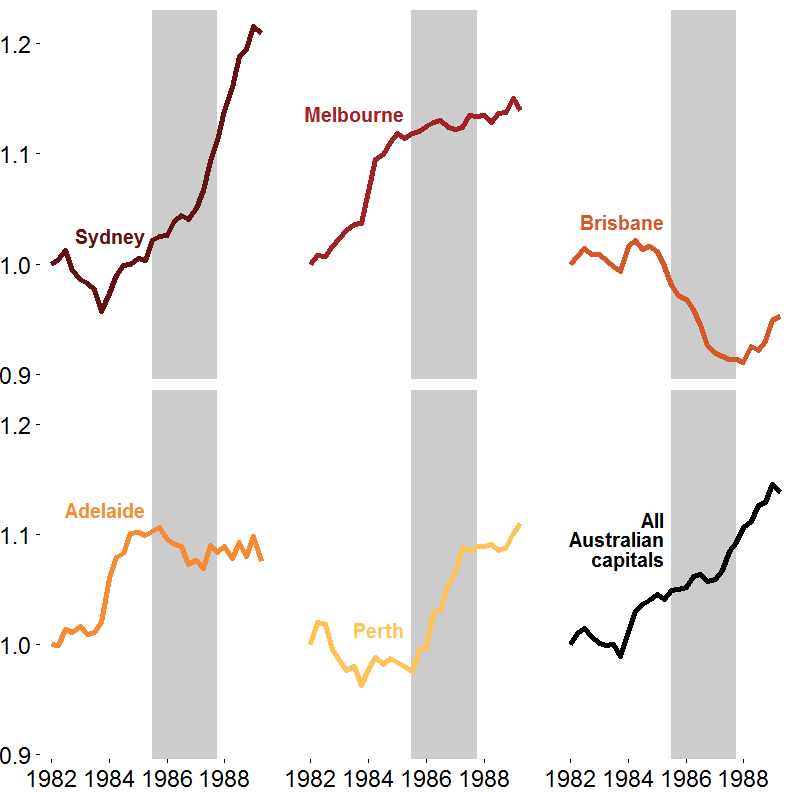
\includegraphics[width=\columnwidth]{CGT-NG-atlas/Capital_city_rents_direct_abs-1}
\source{\textcite{ABSVariousyearsa}}
\end{figure}

The absence of a detectable rental response is also consistent with overseas empirical studies of the relationship between rents and the tax treatment of investment housing. These studies find that rent increases in response to tax changes are modest  and very slow to take effect, with most impacts not seen for more than a decade. 

Beyond these historical lessons, economic theory predicts that limiting negative gearing should not change rents much. 

Limiting or abolishing negative gearing will reduce the post-tax investment returns for negatively geared property investors. There will be a one-off decrease in house prices as investors reduce their willingness to pay. As house prices fall, rental yields -- rents after tax as a proportion of prices -- will rise at least partially restoring the attractiveness of property investment vis- à-vis other investments. 

Existing negatively geared investors will have larger post-tax losses to service. Some may want to increase rents to maintain their returns. But rents are determined by dynamics of demand and supply, not by the returns that owners are seeking. In property markets -- just like other markets -- returns determine asset prices, not the other way around. Rents do not increase just to ensure that buyers of assets get their money back.

Existing negatively geared investors compete to supply rental properties against other property investors with no imperative to increase rents. Rental incomes for the one-third of landlords making positive rental profits would be unaffected by the tax changes. And new investors would purchase properties at lower prices that factor in the less generous tax treatment of rental losses. Tenants can beat rent rises by threatening to move to properties owned by these other investors. 

Some negatively geared investors may sell their properties if tax concessions are less generous. But in the short term this has no impact on rents.  Every time an investor sells a property to a renter, there is one less rental property, and one less renter. There is no change to the balance between supply and demand of rental properties. Others may sell to another investor, but one that doesn't rely on negative gearing to make the investment profitable. Again there is no shortage of rental properties. 

Limiting negative gearing could have an impact on rents over the longer term if lower property prices reduce investment in new rental housing. But the effect is unlikely to be large. Currently 93~per cent of all investment property lending is for existing dwellings.  And one-off price impacts of less than XX per cent (Box 5) are unlikely to substantially slow new construction.  

The main constraint on new housing is land release and zoning restrictions -- especially in established suburbs with good access to jobs and transport.    In housing markets with restricted supply, and where locational factors such as transport links and amenities are important determinants of rental demand, then tax changes have little impact on rents even over time. 



In any case, general tax breaks like negative gearing are an inefficient way of supporting the rental market.\footnote{ 
  The most recent ABS lending data suggests that only 9~percent of recent lending to investors is for constructed properties (ABS Cat. 5671.0 Table 8). One recent paper suggests the 9~percent figure might be understated because the ABS data do not separately identify investor purchase of new housing (as opposed to construction of new housing). Assuming the share of lending for new dwellings by investors is a similar proportion as for owner occupiers, then 12~percent of lending for investment properties would be for new dwellings (either constructed or bought new). }   Blanket tax concessions for investors that primarily accrue to existing property owners through higher house prices are poorly targeted way of alleviating rental stress.  


\subsection{Capping loss deductions}

Capping the total amount of investment losses that can be deducted each
year has been presented as a way to curb the `excesses' of negative
gearing policy.

Capping losses will tend to affect high income earners because they
claim much higher losses on average (section \TBD{3.2}).

The budgetary impact depends on where the cap is set. Table x sets out
the amount of money that could be raised in the longer term if loss
write off against salary and wages is capped annually. Setting a cap on
losses of \$20,000 or more means the policy change will make very little
contribution to the budget bottom line.






\section{\TBD{Number of properties}}

\begin{table}[!h]
\begin{center}
% Jim QC
% eval=FALSE due no access to HILDA
% latex table generated in R 3.5.2 by xtable 1.8-3 package
% Sun Jan 27 15:19:59 2019
\begin{tabularx}{\linewidth}{rr}
  \toprule
{\textbf{Investment properties owned}} & {\textbf{Households}} \\ 
  \midrule
  1 & 376,377 \\ 
    2 & 670,296 \\ 
    3 & 224,579 \\ 
    4 & 120,203 \\ 
    5 & 54,685 \\ 
    6 & 25,331 \\ 
    7 & 9,216 \\ 
    8 & 3,218 \\ 
    9 & 8,674 \\ 
   10 & 2,113 \\ 
   13 & 3,664 \\ 
   14 & 1,790 \\ 
   27 & 6,242 \\ 
   58 & 2,813 \\ 
   & 21,392,249 \\ 
   \bottomrule
\end{tabularx}

\end{center}
\source{HILDA}
\end{table}

\begin{table}
% latex table generated in R 3.5.2 by xtable 1.8-3 package
% Sun Jan 27 15:19:59 2019
\begin{tabularx}{\linewidth}{rr}
  \toprule
  \midrule
0 & 7,631,426 \\ 
  1 & 818,633 \\ 
  2 & 316,366 \\ 
   \bottomrule
\end{tabularx}

\source{Survey Income Housing 2013-14}
\end{table}

\begin{table*}
\caption{Taxpayers with wage and salary income claiming business losses by occupation}\label{tbl:bizlosses}
% latex table generated in R 3.5.2 by xtable 1.8-3 package
% Sun Jan 27 15:20:00 2019
\begin{tabularx}{\linewidth}{lrrrrr}
  \toprule
{\textbf{Occupation}} & {\textbf{Type}} & {\textbf{No. claiming losses}} & {\textbf{\%}} & {\textbf{Average loss}} & {\textbf{Average salary}} \\ 
  \midrule
Clerical and Administrative & Primary & 2450 & 0\% & \$20,154 & \$80,048 \\ 
  Clerical and Administrative & Non-Primary & 19200 & 1\% & \$12,817 & \$50,484 \\ 
   [6pt]Community and Personal Service & Primary & 1300 & 0\% & \$23,243 & \$66,380 \\ 
  Community and Personal Service & Non-Primary & 12400 & 1\% & \$8,029 & \$42,930 \\ 
   [6pt]Consultants, apprentices & Primary & 1450 & 0\% & \$24,215 & \$70,604 \\ 
  Consultants, apprentices & Non-Primary & 7500 & 1\% & \$8,596 & \$59,818 \\ 
   [6pt]Labourers & Primary & 3250 & 0\% & \$30,074 & \$58,522 \\ 
  Labourers & Non-Primary & 8050 & 1\% & \$12,428 & \$47,932 \\ 
   [6pt]Machinery operators and drivers & Primary & 2850 & 0\% & \$31,535 & \$80,644 \\ 
  Machinery operators and drivers & Non-Primary & 6750 & 1\% & \$11,488 & \$56,406 \\ 
   [6pt]Managers & Primary & 5000 & 0\% & \$38,115 & \$131,118 \\ 
  Managers & Non-Primary & 19500 & 2\% & \$14,479 & \$72,434 \\ 
   [6pt]Other & Primary & 0 & 0\% &  &  \\ 
  Other & Non-Primary & 50 & 0\% & \$14,467 & \$13,897 \\ 
   [6pt]Professionals & Primary & 4950 & 0\% & \$39,878 & \$111,882 \\ 
  Professionals & Non-Primary & 39350 & 2\% & \$11,564 & \$67,704 \\ 
   [6pt]Sales & Primary & 650 & 0\% & \$25,238 & \$82,820 \\ 
  Sales & Non-Primary & 9600 & 1\% & \$9,822 & \$42,365 \\ 
   [6pt]Technicians and Trades & Primary & 3900 & 0\% & \$30,661 & \$93,263 \\ 
  Technicians and Trades & Non-Primary & 19400 & 2\% & \$9,068 & \$64,657 \\ 
   \bottomrule
\end{tabularx}

\source{2\%\ sample file 2015-16}
\end{table*}

%\flushcolsend
\chapter{Options for reform}
The favourable tax treatment of investments -- particularly the interaction of the negative gearing arrangements with the capital gains tax discount -- have promoted speculative investment in housing while also costing the budget bottom line. 

Reducing the capital gains tax discount is the most direct way to reduce the incentive for inefficient investment activity. In addition, negative gearing should be restricted so that losses from investments cannot be deducted against wage and salary income. 

Quarantining loss write offs should apply to all types of passive investments, not just rental properties, so that the tax system does not encourage investors to favour one type of investment over another. Similarly, carve outs for negative gearing -- exempting new property, capping total deductions or limiting the number of properties that can be negatively geared -- produce inferior economic outcomes relative to a blanket restriction against deducting losses on investments from wages.

Over the longer term, a more fundamental rethink of the taxation of savings income may be warranted. The proposal from the Henry review to align the tax treatment of savings including interest income, net rental income, capital gains and interest expenses would provide a more consistent treatment of household savings and remains a worthy longer-term policy goal.  Realistically, however, it is not feasible until budget outcomes markedly improve.

\section{Reducing the capital gains tax discount}
The 50 per cent \highlight{capital gains tax (CGT) discount} provides an annual discount to individuals and trusts worth \highlight{\$6-7~billion} annually.

\TBD{\dots}

\section{Limiting negative gearing}
There is also a strong case for quarantining wage and salary income so that losses on investments cannot be deducted from wage and salary income. 
\subsection{In principle, losses on investments shound not be deducted from wage and salary income}
\subsection{How should losses be quarantined?}
\subsection{What losses should be quarantined?}
Quarantining of loss write offs should also apply to negatively geared share market investments, although this is unlikely to be large in practice (section 3.1). The arguments for limiting negative gearing for these investments -- reducing the tax shelter on wages and the tax bias towards speculative investments -- are the same as for negatively geared property. And maintaining a consistent tax treatment across housing and share investments also ensures the tax system does not artificially encourage investors to favour one type of investment over another.  

A more difficult issue is whether there should be additional limits on deducting losses on business activities from wages and salary income.  On balance, these arrangements should be left in place. The losses claimed are relatively small, the activities can be readily distinguished from investment losses, and the policy justification is at least plausible. Nevertheless, some features of these losses suggest that the specific rules could be tightened further as many of the losses being claimed may be funding lifestyle expenses rather than attempts to set up sustainable businesses. 

Currently there are more restrictions on deducting business losses than there are on deducting losses from investments. Sole traders and participants in a partnership can write off losses from these business activities against unrelated income (including wages) only if they meet a variety of conditions that generally exclude activities that make persistent losses.  Losses for incorporated businesses cannot be written off against other income. 



The losses claimed are relatively small. In 2015-16 only 250,000~taxpayers claimed \$4~billion in business losses (compared to 1.3~million claiming \$10~billion in losses on property).

\TBD{\dots}



\begin{figure}
\Caption{Those earning more claim bigger primary production losses}{Salary}{fig:PP-losses-by-occ}











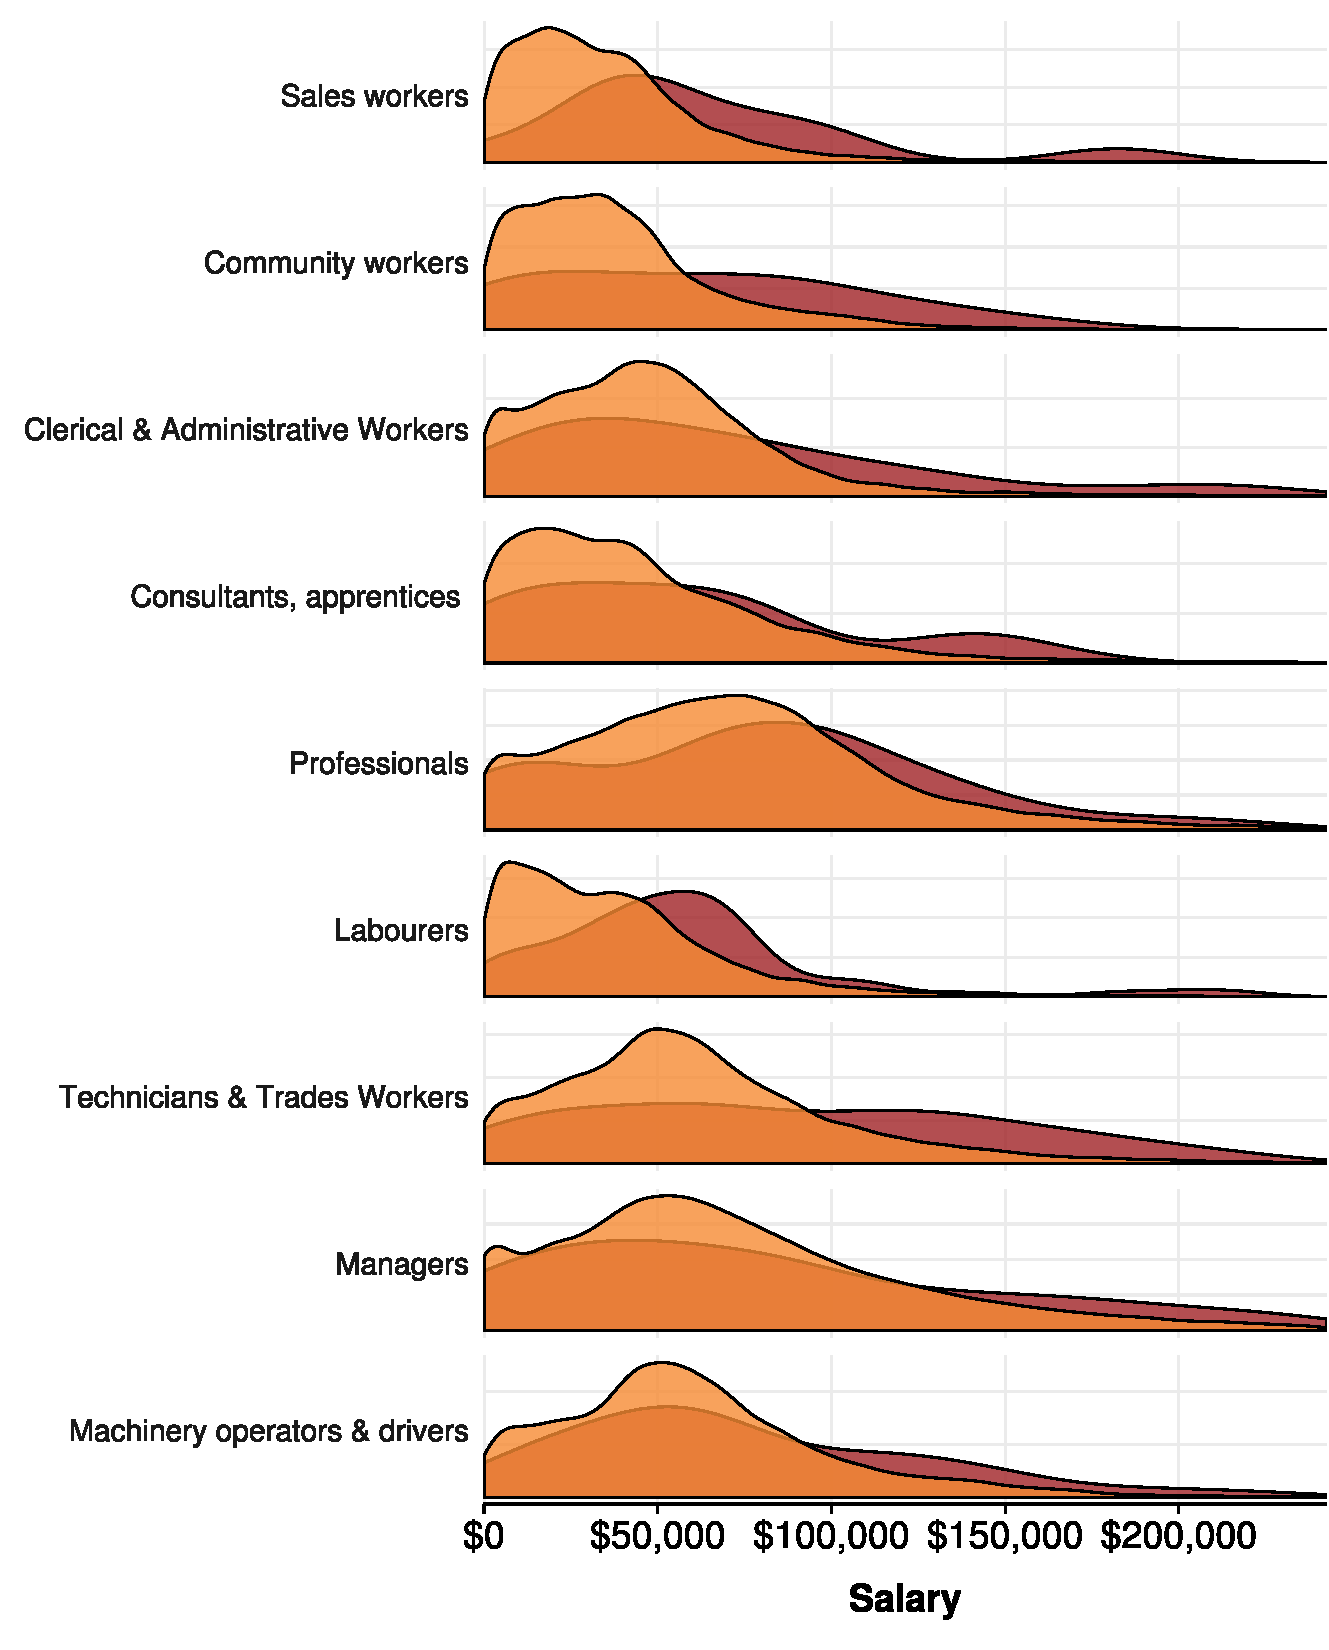
\includegraphics[width=\columnwidth]{CGT-NG-atlas//density-salary-by-PP-losses-1}
\end{figure}

\begin{figure}
\Caption{Relative salaries are higher for those earning PP}{Salary, 2015-16}{fig:density-salary-by-PP-losses}
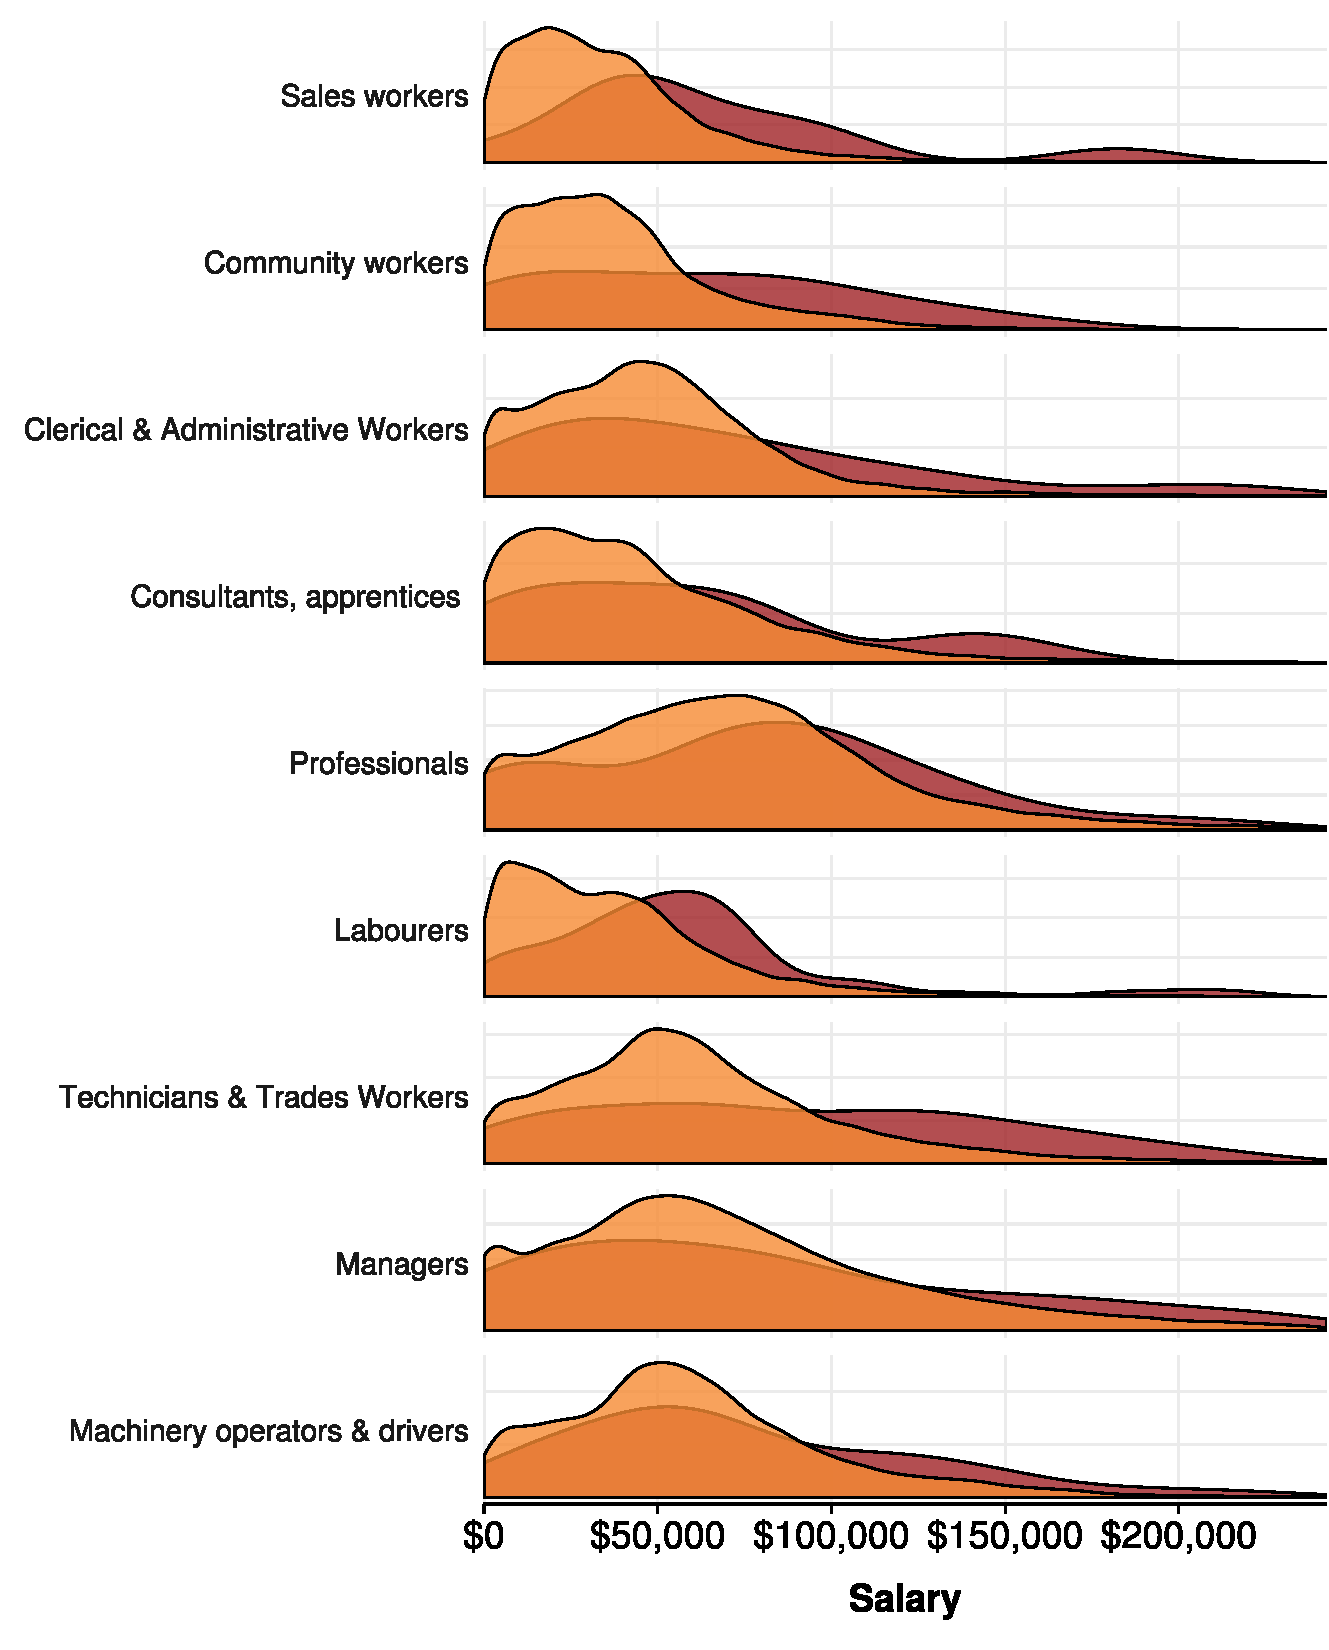
\includegraphics[width=\columnwidth]{CGT-NG-atlas//density-salary-by-PP-losses-1}
\end{figure}

However, many of the losses being claimed may not serve this policy purpose. Around 40~percent of business losses claimed are from primary production -- for example, animal or crop farming, vineyards or animal breeding. 45,000~taxpayers claimed \$1.6~billion  in primary production losses -- almost \$40,000 per claimant. In all occupational categories, average salaries for those claiming primary production losses were substantially higher -- between 21~percent and 64~percent -- than the average salaries for their occupation. And the largest tax breaks were for the highest income professions  suggesting that the primary production activity may often be more a lifestyle activity, such as a hobby farm, than a sustainable business. 



About 200,000 taxpayers claimed an average of \$14,000 of non-farm business losses. It is likely that many of these people were individual contractors in fields related to their main job. Some of the losses may simply be taxpayers claiming lifestyle costs where they will be less scrutinised. Tax returns require less detail for costs claimed as part of running a business rather than in incurring wage and salary income (for example, travel costs do not need to be separately disclosed). 



Nevertheless, given the low costs and potentially meaningful benefits the best approach is probably to leave the current tax treatment for losses from unincorporated businesses in place. In other words, only losses from passive investments would be quarantined so they cannot be written off against and wage and salary income. This approach is in place in the United States \TBD{(Appendix C)}. 

\subsubsection{Budget impact}
Restricting negative gearing by quarantining loss deductions for passive investments would raise additional tax revenue, although the estimates depend on future housing prices and how long investors hold their assets. 

For most investors, the changes will mainly affect the timing, not the amount, of tax deductions. The costs of property and share investments will still be deducted against investment income, including subsequent capital gains, although the tax rate applied to some costs will include the CGT discount. 

\begin{knitrout}
\definecolor{shadecolor}{rgb}{0.969, 0.969, 0.969}\color{fgcolor}\begin{kframe}
\begin{verbatim}
## [1] 2982084886
\end{verbatim}
\end{kframe}
\end{knitrout}

We estimate that quarantining losses for passive investments would increase income tax collections by \$2.27~billion a year in the short term. Over the medium term, accrued losses -- losses not offset against recurrent investment income -- will be deducted from capital gains. Assuming no change in investor behaviour, the additional tax revenue would stabilise at around \$1.48~billion a year.

If deductions were limited even more to the particular asset or asset class, income tax collections would rise a little more because investors would wait longer on average until they could realise their losses. 

These estimates do not take into account the effects of investors changing their behaviour in response to the policy change. Investments that make income losses are less attractive when the tax benefits are smaller. Negative gearing appeals largely because it can reduce taxes on wage income (\cref{negative-gearing-provides-a-widely-used-tax-shelter-on-wages}, \Vref{box:NG-to-reduce-tax-on-wages}). Removing the tax incentive for highly leveraged investment should result in investors shifting toward income-producing assets and could therefore further increase income tax collections. On the other hand, if some investment properties are replaced by owner-occupied properties, there will be less revenue collected, because no tax is paid on capital gains on the family home, or on the `imputed rent' -- the value of living in occupier-owned housing.

\section{Alternative policies for limiting negative gearing}
Our proposed policy of quarantining investment losses from wage and salary income would apply to losses from all passive investments regardless of the nature or the size of the investment. 

Others have proposed less universal changes. For example, Labor's negative gearing policy would allow unrestricted loss write offs for new housing.  It was reported in 2016 that the Coalition contemplated policies to cap loss deductions or limit the number of properties that could be negatively geared. 

These `half way house' policies tend to be sub-optimal. The economic arguments for limiting negative gearing apply regardless of investment size or type. By limiting the changes some of the potential budgetary benefits are lost. And introducing differential tax treatments based on the size or type of investment further increases complexity and distorts investment decisions. 

Nevertheless, limiting negative gearing to new properties or capping loss deductions at modest levels may not impose large costs on the budget or the economy. If these carve outs make changes to negative gearing more politically palatable they may still be worthwhile.

On the other hand, capping the number of properties that can be negatively geared or setting a high threshold for loss deductions, eliminate almost all the revenue gains from policy change while introducing additional distortions. 

\subsection{Limiting negative gearing only to new properties}
It would be possible to quarantine wage and salary income generally, but to allow losses on new properties to be deducted from wages and salaries. 

Proponents argue that this exemption will maintain the incentives for the provision of new housing.  But in practice it won't make much difference: most of the tax benefits will be reflected in a one of increase in the price of developable land. The supply of land for development is not particularly responsive to price changes as discussed in section 4.4. Therefore the profits to any favourable tax change affected new development will mainly flow to the landholders. 



In any case, the benefits of negative gearing are likely to be small relative to the price of property and the cost of development -- around XX per cent of the property value.  Even if all of this benefit flowed to developers and purchasers, not to the owners of land suitable for development, there wouldn't be much additional development activity. And of course the impact on overall housing supply would be smaller again because few additional properties are built in any year relative to the stock of existing properties. 

Restricting tax benefits to a subset of investments, such as new housing, creates additional complexity and distorts investment choices. But the costs may not be high. Administrative issues such as how to define `new properties' have already been addressed through  other government support schemes targeting new property investments such as first home buyer's grants and stamp duty concessions. 

And there are clear political benefits from such an exemption.  It appeals to intuitions that tax benefits will result in additional new housing, even if theory and history suggest that the effects will be small.  As the additional costs are low, it may be a political price worth paying.

\subsection{Capping loss deductions}
Capping the total amount of losses that can be deducted each year for negatively geared properties has been proposed as a way to curb the `excesses' of negative gearing policy. 

\begin{figure}
\Caption{Those on high salaries are much more likely to be negatively gearing}{Incidence of negative gearing}{fig:NG-vs-salary}
% dev omit emf due to alpha

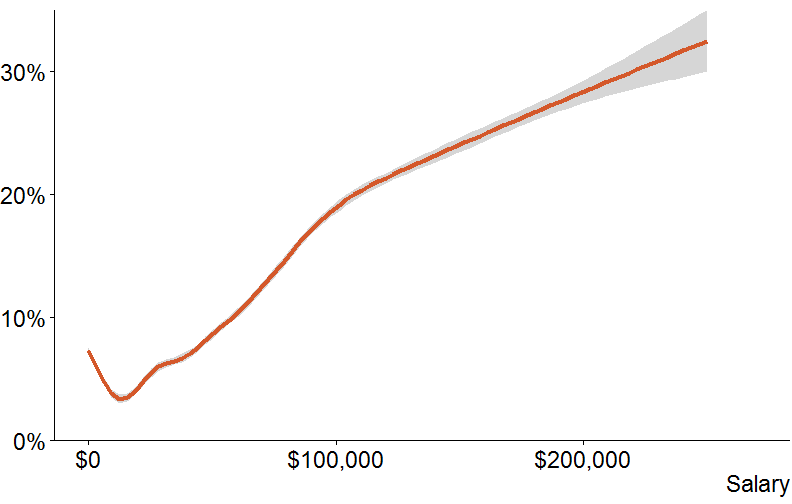
\includegraphics[width=\columnwidth]{CGT-NG-atlas//NG-vs-salary-1}
\end{figure}

Capping losses is politically attractive because a smaller percentage of landlords will be impacted by the policy. And the landlords affected are more likely to be high income earners because those on high incomes claim much higher losses on average (\Vref{fig:NG-vs-salary}). 

\begin{table}
\caption{Budgetary impact of caps to negative gearing}\label{tbl:cap-NG}
% latex table generated in R 3.5.2 by xtable 1.8-3 package
% Sun Jan 27 15:20:15 2019
\begin{tabularx}{\linewidth}{rrrS}
  \toprule
{\textbf{Threshold}} & {\textbf{Costing}} & {\textbf{Number affected}} & {\textbf{\%}} \\ 
  \midrule
$-$\$50,000 & \$46,831,392 & 7,343 & 0\% \\ 
  $-$\$20,000 & \$338,933,623 & 72,443 & 4\% \\ 
  $-$\$15,000 & \$518,432,512 & 121,711 & 6\% \\ 
  $-$\$10,000 & \$832,498,426 & 222,330 & 11\% \\ 
  $-$\$5,000 & \$1,411,118,007 & 416,172 & 21\% \\ 
  $-$\$0 & \$2,483,067,238 & 770,576 & 38\% \\ 
   \bottomrule
\end{tabularx}

\end{table}


The budget impact will depend on the level of the cap, as set out in \Vref{tbl:cap-NG}. A cap on losses of \$20,000  would affect very few landlords, and would make very little difference to the budget bottom line.

An alternative is to limit deductions. This could apply to all deductions including work related expenses, interest costs, donations etc. This would ultimately impose a minimum effective rate of tax for high income earners.   A full consideration of such a proposal is beyond the scope of this report. 

\subsection{Limits on number of properties}
An alternative proposal would limit the number of properties on which investors are able to claim losses.  This is an unattractive option. It would raise little, is poorly targeted, and would increase the distortions in the housing market.



Only 31~percent of landlords have two or more properties.  A fraction of these would not be taxed as they would the `first property' for a landlord. The relatively small number of taxpayers affected substantially reduces the potential budget gains. 

In any case, capping property numbers is a crude way to target `excessive' negative gearing. Taxpayers can increase their deductions by purchasing fewer but more expensive properties. Consequently the policy will distort investment decisions by discouraging investors from buying more affordable properties. 

\section{Summarising impact of proposed negative gearing and CGT changes}
Our preferred policy is to reduce the CGT discount to 25~percent and limit negative gearing by quarantining all passive investment losses. 

In addition to raising more than \$5.33~billion a year, these changes will reduce (although not eliminate) distortions in investment choices toward debt financing of investment. Effective tax rates will increase a bit more for highly leveraged investors because they lose some of the tax benefits of upfront loss write offs \TBD{(Figure 18)}. However, effective tax rates will remain lower for this group because they still eventually write off their losses at a tax rate higher than they pay on gains. 

\chapter{Transition arrangements}




\begin{knitrout}
\definecolor{shadecolor}{rgb}{0.969, 0.969, 0.969}\color{fgcolor}\begin{kframe}
\begin{verbatim}
## [1] 0.187
\end{verbatim}
\end{kframe}
\end{knitrout}
\begin{figure}
\Caption{Negative gearing spells are short}{Survival curve of negative gearing responding persons}{fig:NG-spells-are-short}

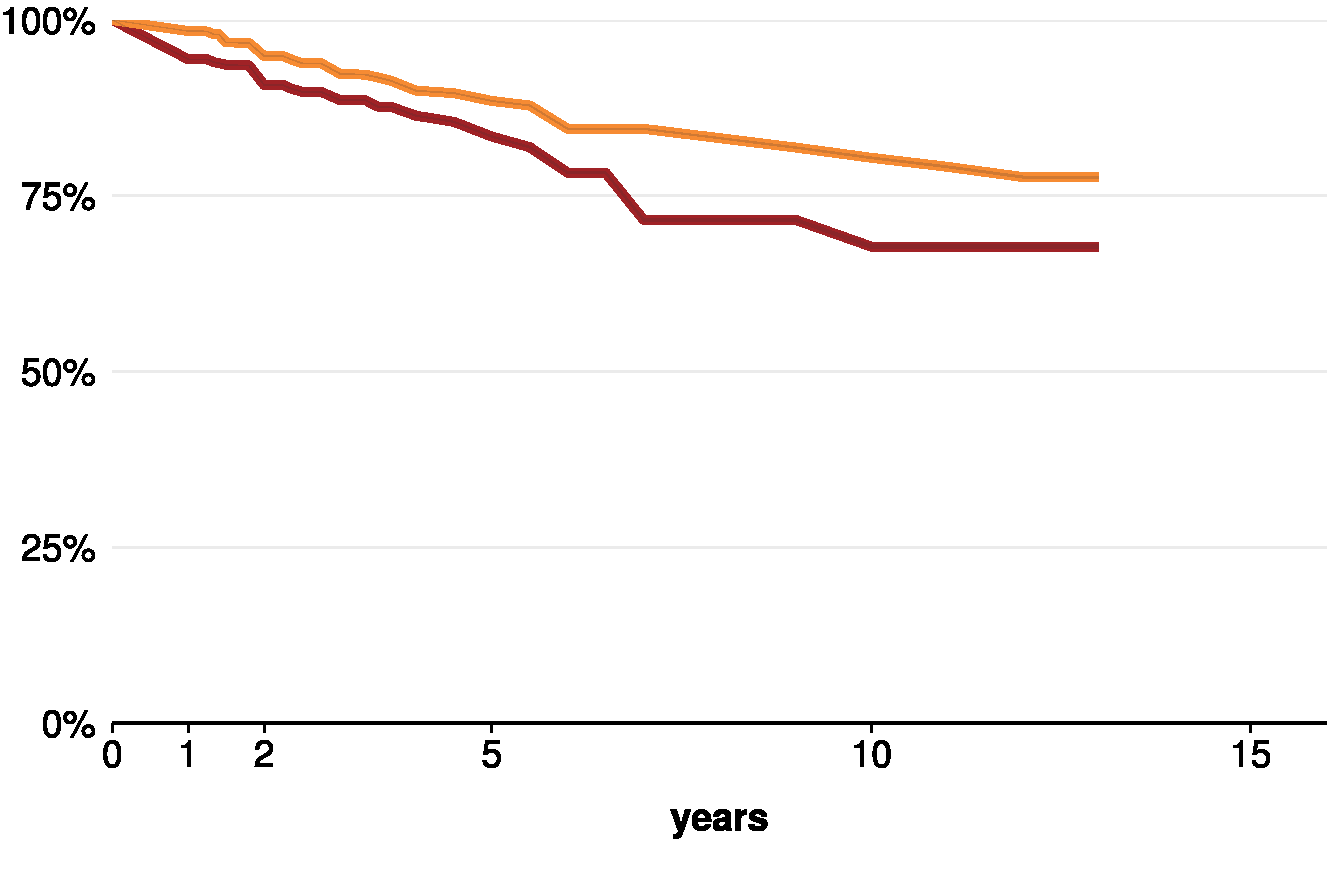
\includegraphics[width=\columnwidth]{CGT-NG-atlas//NG-survival-curve-1}
\notes{Probably wrong: Individuals suffering from left- or right-censoring were simply omitted!}

\source{HILDA}
\end{figure}
\printbibliography[title=References]


\appendix
\chapter{Capital gains tax and asset lock-in}
One reason often provided for lower taxes on capital gains is to reduce ``asset lock-in''. If investors are less likely to realise gains when tax rates are higher than increasing taxes on gains could actually reduce tax collections in the short to medium term. But the empirical evidence of lock-in in not settled. In Australia, the primary driver of asset lock-in appears to be people waiting until retirement to sell their assets. This incentive is still strong even with a 50 per cent discount. 

\section{Why does asset lock-in occur?}
Asset lock-in occurs because taxes are only paid when gains are realised. This provides an incentive for investors to hold on to assets with large accumulated gains.  In effect, the investor seeks to maintain the implicit interest free loan on accrued gains. Crystallising a capital gain is only worthwhile if an investor can achieve a materially higher return elsewhere, or if they want the resources for consumption (\Vref{box:CGT-asset-lock-in}).   

Lock-in can discourage investors from moving their money to the investments with the highest pre-tax returns, so assets do not always go to their highest value use.  Lock-in effects are most significant from a whole of economy perspective, if they constrain financing of profitable investments.  

\begin{smallbox}[!htbp]{Capital gains tax and asset lock-in}{box:CGT-asset-lock-in}
The tax treatment of capital gains can deter investors from taking up otherwise profitable investment opportunities. 



Suppose Hayley, an investor in the top tax bracket purchases a house for \$700,000 and holds it for 10 years. During that time the market price of the house increases to \$1,000,000. She makes a net rental return of 5~percent a year, so her  final income is \$50,000. 

If she were to sell the house she would crystallise the \$300,000 in gains, paying tax on 50~percent of the gains at her marginal tax rate of 49~percent (\$73,500). This would leave her with around \$926,500 from the sale: \$226,500 in net gains and her initial investment of \$700,000. 

The sale will only be worthwhile if Hayley can find an alternative property that yields more than her current rental income of \$50,000  with the same opportunity for capital gains. With her \$926,500 sale proceeds she would need to find a property with net rental return of more than 5~percent a year. 

Properties with rental yields below 5~percent but higher than her current 5 would not be attractive because realising the tax liability on her current property erodes her capital base for investment.  

The higher the tax rate on capital gains the less willing she will be to realise gains to pursue new investment opportunities. If capital gains were taxed in full, rather than with a 50 per cent discount, her hurdle rate for the new investment would be 6~percent.
\end{smallbox}

% For longtable.
\onecolumn
\chapter{International comparisons of capital gains tax}
Internationally, there are a range of approaches to taxing capital gains. Most countries offer some form of tax discount for capital income but the amount of the discount and the holding period to qualify vary widely. Contrary to the claims of some, taxes on capital gains are more concessional than in many other OECD countries (vide infra).

\newcommand{\cella}[1]{{\cellcolor{Color2}\makecell[tr]{#1}}}
\newcommand{\cellb}[1]{{\cellcolor{Color3}\makecell[tr]{#1}}}
\newcommand{\cellc}[1]{\cellcolor{Color4}\makecell[tr]{#1}}
\newcommand{\celld}[1]{\cellcolor{Color5}\makecell[tr]{#1}}

\renewcommand{\arraystretch}{1.2}
\begin{longtable}{lrrrrrr}
\toprule
 & \multicolumn{2}{c}{Property} & \multicolumn{2}{c}{Shares} &  & \\
 \cmidrule(lr){2-3}\cmidrule(lr){4-5} 
 Country & CGT & Holding test? & CGT & Holding test? & Top MTR & Adj for inflation? \\ 
 \midrule
 \endhead
 \bottomrule
 \endfoot
 Australia & \cellcolor{Color3}{50\%\ exempt, rest at MTR} & \cellcolor{Color3}{1\,yr} & \cellcolor{Color3}{50\%\ exempt, rest at MTR} & \cellb{1\,yr} & 47 & N\\ 
 Austria   & \cellc{Progressive rise to 50\% from 10-35 years,\\ rest at MTR} & \cellcolor{Color4}10-35\,yr & \cellcolor{Color4} 25\% exempt, rest at MTR & -- & \cellcolor{Color3}{50} & \cellcolor{Color3}{N} \\ 
 Australia & 50\%\ exempt, rest at MTR & 1\,yr & 50\%\ exempt, rest at MTR & 1 yr \\ 
 Australia & 50\%\ exempt, rest at MTR & 1\,yr & 50\%\ exempt, rest at MTR & 1 yr \\ 
 Australia & 50\%\ exempt, rest at MTR & 1\,yr & 50\%\ exempt, rest at MTR & 1 yr \\ 
 Australia & 50\%\ exempt, rest at MTR & 1\,yr & 50\%\ exempt, rest at MTR & 1 yr \\ 
 Australia & 50\%\ exempt, rest at MTR & 1\,yr & 50\%\ exempt, rest at MTR & 1 yr \\ 
 Australia & 50\%\ exempt, rest at MTR & 1\,yr & 50\%\ exempt, rest at MTR & 1 yr \\ 
 Australia & 50\%\ exempt, rest at MTR & 1\,yr & 50\%\ exempt, rest at MTR & 1 yr \\ 
 Australia & 50\%\ exempt, rest at MTR & 1\,yr & 50\%\ exempt, rest at MTR & 1 yr \\ 
 Australia & 50\%\ exempt, rest at MTR & 1\,yr & 50\%\ exempt, rest at MTR & 1 yr \\ 
 Australia & 50\%\ exempt, rest at MTR & 1\,yr & 50\%\ exempt, rest at MTR & 1 yr \\ 
 Australia & 50\%\ exempt, rest at MTR & 1\,yr & 50\%\ exempt, rest at MTR & 1 yr \\ 
 Australia & 50\%\ exempt, rest at MTR & 1\,yr & 50\%\ exempt, rest at MTR & 1 yr \\ 
 Australia & 50\%\ exempt, rest at MTR & 1\,yr & 50\%\ exempt, rest at MTR & 1 yr \\ 
 Australia & 50\%\ exempt, rest at MTR & 1\,yr & 50\%\ exempt, rest at MTR & 1 yr \\ 
 Australia & 50\%\ exempt, rest at MTR & 1\,yr & 50\%\ exempt, rest at MTR & 1 yr \\ 
 Australia & 50\%\ exempt, rest at MTR & 1\,yr & 50\%\ exempt, rest at MTR & 1 yr \\ 
 Australia & 50\%\ exempt, rest at MTR & 1\,yr & 50\%\ exempt, rest at MTR & 1 yr \\ 
 Australia & 50\%\ exempt, rest at MTR & 1\,yr & 50\%\ exempt, rest at MTR & 1 yr \\ 
 Australia & 50\%\ exempt, rest at MTR & 1\,yr & 50\%\ exempt, rest at MTR & 1 yr \\ 
 Australia & 50\%\ exempt, rest at MTR & 1\,yr & 50\%\ exempt, rest at MTR & 1 yr \\ 
 Australia & 50\%\ exempt, rest at MTR & 1\,yr & 50\%\ exempt, rest at MTR & 1 yr \\ 
 Australia & 50\%\ exempt, rest at MTR & 1\,yr & 50\%\ exempt, rest at MTR & 1 yr \\ 
 Australia & 50\%\ exempt, rest at MTR & 1\,yr & 50\%\ exempt, rest at MTR & 1 yr \\ 
 Australia & 50\%\ exempt, rest at MTR & 1\,yr & 50\%\ exempt, rest at MTR & 1 yr \\ 
 Australia & 50\%\ exempt, rest at MTR & 1\,yr & 50\%\ exempt, rest at MTR & 1 yr \\ 
 Australia & 50\%\ exempt, rest at MTR & 1\,yr & 50\%\ exempt, rest at MTR & 1 yr \\ 
 Australia & 50\%\ exempt, rest at MTR & 1\,yr & 50\%\ exempt, rest at MTR & 1 yr \\ 
 Australia & 50\%\ exempt, rest at MTR & 1\,yr & 50\%\ exempt, rest at MTR & 1 yr \\ 
%\bottomrule
\end{longtable}
\renewcommand{\arraystretch}{1.0}
\twocolumn
\chapter{Effective tax rates by investment return and tax bracket}
Effective tax rates measure the tax paid on investment returns as a share of the pre-tax returns. Effective tax rates vary by the investor’s tax rate and the level of returns. When looking at effective tax rate on real returns (returns adjusted for inflation) or on `excess returns' (returns above the risk free rate) the level of inflation and the returns will also affect the effective tax rate paid by the investor. 

\Vref{fig:EMTR-savings} presents effective rates for two different return scenarios for an investor in the 47\,c tax bracket. \Vref{tbl:Real-EMTR-appendix} below presents calculations for a broader range of return scenarios and investor tax brackets. 







\begin{table*}
\centering
\captionsetup{justification=centering}
\caption[Effective marginal tax rates for a rental property]{Effective marginal tax rates for a rental property}\label{tbl:Real-EMTR-appendix}
\newcolumntype{Q}{@{}l@{}}
\begin{tikzpicture}
\begin{ocg}{ocgBlack}{ocgBlack}{1}
 \node (BlackNode) {%


% latex table generated in R 3.5.2 by xtable 1.8-3 package
% Sun Jan 27 15:21:25 2019
\begin{tabular}{Qlllrrrrr}
  \toprule
   &  &  &  & \multicolumn{5}{c}{\textbf{Nominal annual capital gain}}\\
 \cmidrule(lr){5-9}
 \textbf{\phantom{.}} & \textbf{Marginal tax rate} & \textbf{Return type} & \textbf{CGT treatment} & \textbf{4.0\%} & \textbf{5.0\%} & \textbf{6.0\%} & \textbf{8.0\%} & \textbf{10.0\%}\\
 \midrule
 & 34.5 & real & 50\% discount & 33.9 & 29.4 & 26.2 & 21.7 & 18.7 \\ 
   &  &  & Indexed & 34.3 & 32.6 & 31.1 & 28.5 & 26.2 \\ 
   &  &  & 25\% discount & 39.6 & 35.0 & 31.7 & 26.9 & 23.6 \\ 
   &  &  & 0\% discount & 45.5 & 40.9 & 37.4 & 32.4 & 28.8 \\ 
  &\phantom{.}\\[-9pt] &  & excess & 50\% discount & 61.0 & 46.2 & 37.8 & 28.4 & 23.1 \\ 
   &  &  & Indexed & 61.7 & 51.2 & 44.9 & 37.2 & 32.4 \\ 
   &  &  & 25\% discount & 71.3 & 55.1 & 45.8 & 35.2 & 29.1 \\ 
   &  &  & 0\% discount & 82.0 & 64.3 & 54.1 & 42.4 & 35.5 \\ 
  &\phantom{.}\\[-6pt] & 39.0 & real & 50\% discount & 38.5 & 33.4 & 29.8 & 24.7 & 21.3 \\ 
   &  &  & Indexed & 38.8 & 37.0 & 35.4 & 32.5 & 30.0 \\ 
   &  &  & 25\% discount & 45.1 & 39.9 & 36.1 & 30.7 & 27.0 \\ 
   &  &  & 0\% discount & 51.9 & 46.7 & 42.8 & 37.1 & 33.1 \\ 
  &\phantom{.}\\[-9pt] &  & excess & 50\% discount & 69.2 & 52.5 & 43.0 & 32.3 & 26.3 \\ 
   &  &  & Indexed & 69.8 & 58.1 & 51.1 & 42.5 & 37.1 \\ 
   &  &  & 25\% discount & 81.1 & 62.7 & 52.2 & 40.2 & 33.3 \\ 
   &  &  & 0\% discount & 93.5 & 73.4 & 61.9 & 48.6 & 40.9 \\ 
  &\phantom{.}\\[-6pt] & 47.0 & real & 50\% discount & 46.7 & 40.6 & 36.2 & 30.1 & 26.0 \\ 
   &  &  & Indexed & 46.8 & 44.8 & 43.1 & 39.9 & 37.1 \\ 
   &  &  & 25\% discount & 54.9 & 48.8 & 44.2 & 37.7 & 33.2 \\ 
   &  &  & 0\% discount & 63.6 & 57.4 & 52.8 & 46.0 & 41.1 \\ 
  &\phantom{.}\\[-9pt] &  & excess & 50\% discount & 84.0 & 63.8 & 52.3 & 39.4 & 32.1 \\ 
   &  &  & Indexed & 84.2 & 70.5 & 62.2 & 52.2 & 45.8 \\ 
   &  &  & 25\% discount & 98.9 & 76.6 & 63.8 & 49.3 & 41.0 \\ 
   &  &  & 0\% discount & 114.5 & 90.2 & 76.2 & 60.2 & 50.8 \\ 
   \bottomrule
\end{tabular}

};%
\end{ocg}
\begin{ocg}{ocgColored}{ocgColored}{0}
\node (Coloured) {%
% latex table generated in R 3.5.2 by xtable 1.8-3 package
% Sun Jan 27 15:21:25 2019
\begin{tabular}{Qlllrrrrr}
  \toprule
   &  &  &  & \multicolumn{5}{c}{\textbf{Nominal annual capital gain}}\\
 \cmidrule(lr){5-9}
 \textbf{Marginal tax rate} & \textbf{Return type} & \textbf{CGT treatment} & \textbf{\phantom{.}} & \textbf{4.0\%} & \textbf{5.0\%} & \textbf{6.0\%} & \textbf{8.0\%} & \textbf{10.0\%}\\
 \midrule
 &  & 0\% discount &  & \cellcolor{Color3}{45.5} & \cellcolor{Color3}{40.9} & \cellcolor{Color3}{37.4} & \cellcolor{Color2}{32.4} & \cellcolor{Color2}{28.8} \\ 
   &  & 0\% discount &  & \cellcolor{Color5}{82.0} & \cellcolor{Color4}{64.3} & \cellcolor{Color4}{54.1} & \cellcolor{Color3}{42.4} & \cellcolor{Color3}{35.5} \\ 
   &  & 0\% discount &  & \cellcolor{Color4}{51.9} & \cellcolor{Color3}{46.7} & \cellcolor{Color3}{42.8} & \cellcolor{Color3}{37.1} & \cellcolor{Color2}{33.1} \\ 
   &  & 0\% discount &  & \cellcolor{Color6}{93.5} & \cellcolor{Color5}{73.4} & \cellcolor{Color4}{61.9} & \cellcolor{Color3}{48.6} & \cellcolor{Color3}{40.9} \\ 
   &  & 0\% discount &  & \cellcolor{Color4}{63.6} & \cellcolor{Color4}{57.4} & \cellcolor{Color4}{52.8} & \cellcolor{Color3}{46.0} & \cellcolor{Color3}{41.1} \\ 
   &  & 0\% discount &  & \cellcolor{black}{\textcolor{white}{114.5}} & \cellcolor{Color6}{90.2} & \cellcolor{Color5}{76.2} & \cellcolor{Color4}{60.2} & \cellcolor{Color4}{50.8} \\ 
   &  & 25\% discount &  & \cellcolor{Color3}{39.6} & \cellcolor{Color3}{35.0} & \cellcolor{Color2}{31.7} & \cellcolor{Color2}{26.9} & \cellcolor{Color2}{23.6} \\ 
   &  & 25\% discount &  & \cellcolor{Color5}{71.3} & \cellcolor{Color4}{55.1} & \cellcolor{Color3}{45.8} & \cellcolor{Color3}{35.2} & \cellcolor{Color2}{29.1} \\ 
   &  & 25\% discount &  & \cellcolor{Color3}{45.1} & \cellcolor{Color3}{39.9} & \cellcolor{Color3}{36.1} & \cellcolor{Color2}{30.7} & \cellcolor{Color2}{27.0} \\ 
   &  & 25\% discount &  & \cellcolor{Color5}{81.1} & \cellcolor{Color4}{62.7} & \cellcolor{Color4}{52.2} & \cellcolor{Color3}{40.2} & \cellcolor{Color2}{33.3} \\ 
   &  & 25\% discount &  & \cellcolor{Color4}{54.9} & \cellcolor{Color3}{48.8} & \cellcolor{Color3}{44.2} & \cellcolor{Color3}{37.7} & \cellcolor{Color2}{33.2} \\ 
   &  & 25\% discount &  & \cellcolor{Color6}{98.9} & \cellcolor{Color5}{76.6} & \cellcolor{Color4}{63.8} & \cellcolor{Color3}{49.3} & \cellcolor{Color3}{41.0} \\ 
   &  & Indexed &  & \cellcolor{Color3}{34.3} & \cellcolor{Color2}{32.6} & \cellcolor{Color2}{31.1} & \cellcolor{Color2}{28.5} & \cellcolor{Color2}{26.2} \\ 
   &  & Indexed &  & \cellcolor{Color4}{61.7} & \cellcolor{Color4}{51.2} & \cellcolor{Color3}{44.9} & \cellcolor{Color3}{37.2} & \cellcolor{Color2}{32.4} \\ 
   &  & Indexed &  & \cellcolor{Color3}{38.8} & \cellcolor{Color3}{37.0} & \cellcolor{Color3}{35.4} & \cellcolor{Color2}{32.5} & \cellcolor{Color2}{30.0} \\ 
   &  & Indexed &  & \cellcolor{Color5}{69.8} & \cellcolor{Color4}{58.1} & \cellcolor{Color4}{51.1} & \cellcolor{Color3}{42.5} & \cellcolor{Color3}{37.1} \\ 
   &  & Indexed &  & \cellcolor{Color3}{46.8} & \cellcolor{Color3}{44.8} & \cellcolor{Color3}{43.1} & \cellcolor{Color3}{39.9} & \cellcolor{Color3}{37.1} \\ 
   &  & Indexed &  & \cellcolor{Color6}{84.2} & \cellcolor{Color5}{70.5} & \cellcolor{Color4}{62.2} & \cellcolor{Color4}{52.2} & \cellcolor{Color3}{45.8} \\ 
   & excess & 50\% discount & &\phantom{.}\\[-9pt] & \cellcolor{Color4}{61.0} & \cellcolor{Color3}{46.2} & \cellcolor{Color3}{37.8} & \cellcolor{Color2}{28.4} & \cellcolor{Color2}{23.1} \\ 
   & excess & 50\% discount & &\phantom{.}\\[-9pt] & \cellcolor{Color5}{69.2} & \cellcolor{Color4}{52.5} & \cellcolor{Color3}{43.0} & \cellcolor{Color2}{32.3} & \cellcolor{Color2}{26.3} \\ 
   & excess & 50\% discount & &\phantom{.}\\[-9pt] & \cellcolor{Color6}{84.0} & \cellcolor{Color4}{63.8} & \cellcolor{Color4}{52.3} & \cellcolor{Color3}{39.4} & \cellcolor{Color2}{32.1} \\ 
  34.5 & real & 50\% discount &  & \cellcolor{Color3}{33.9} & \cellcolor{Color2}{29.4} & \cellcolor{Color2}{26.2} & \cellcolor{Color2}{21.7} & \cellcolor{Color2}{18.7} \\ 
  39.0 & real & 50\% discount & &\phantom{.}\\[-6pt] & \cellcolor{Color3}{38.5} & \cellcolor{Color3}{33.4} & \cellcolor{Color2}{29.8} & \cellcolor{Color2}{24.7} & \cellcolor{Color2}{21.3} \\ 
  47.0 & real & 50\% discount & &\phantom{.}\\[-6pt] & \cellcolor{Color3}{46.7} & \cellcolor{Color3}{40.6} & \cellcolor{Color3}{36.2} & \cellcolor{Color2}{30.1} & \cellcolor{Color2}{26.0} \\ 
   \bottomrule
\end{tabular}

};%
\end{ocg}
\end{tikzpicture}
\footnotesize
\begin{tabular}{lp{0.5\textwidth}}
\footnotesize Notes: & {\footnotesize Inflation 2.5\%. Property earns 3\%\ nominal rent in addition to the capital growth and which is reinvested in the property till maturity. Risk free rate 4.5\%. Property is held for 15 years then disposed and capital gain realized without losses.\hfill{\switchocg{ocgBlack ocgColored}{\textcolor{DarkOrange}{\textbf{Click to colour cells.}}}}}
\end{tabular}
\end{table*}


\onecolumn
\chapter{Session info of $\mathsf{R}$ used for compilation}
\begin{multicols*}{2}
This report was woven from  \textrm{\LaTeX2e} and $\mathsf{R}$ by \textbf{knitr}. 

\textrm{\LaTeX2e} is a document preparation system implemented as a macro package for Donald E.\ Knuth's \textrm{\TeX} typesetting program. \textrm{\LaTeX} was originally conceived by Leslie Lamport. 

$\mathsf{R}$ is a language and environment for statistical computing derived from the S programming language of John Chambers. $\mathsf{R}$ was created by Ross Ihaka and Robert Gentlement at the University of Auckland. 

\textbf{knitr} a general-purpose package for dynamic, literate report generation in $\mathsf{R}$ developed from Sweave. Yihui Xie is the author and developer of \textbf{knitr}. 

The authors are indebted to the creators.

The \verb=devtools::session_info()= is printed below.
% \eject
% \phantom{.}
% \vfill
% \phantom{.}
\end{multicols*}


\begin{table*}[!htb]
\centering
\caption{Platform}
% latex table generated in R 3.5.2 by xtable 1.8-3 package
% Sun Jan 27 15:21:26 2019
\begin{tabularx}{\linewidth}{l}
  \toprule
 R version 3.5.2 (2018-12-20) \\ 
  Windows 10 x64 \\ 
  x86\_64, mingw32 \\ 
  RTerm \\ 
  (EN) \\ 
  English\_Australia.1252 \\ 
  English\_Australia.1252 \\ 
  Australia/Sydney \\ 
  2019-01-27 \\ 
   \bottomrule
\end{tabularx}

\end{table*}

% for longtable



% latex table generated in R 3.5.2 by xtable 1.8-3 package
% Sun Jan 27 15:21:27 2019
\begin{longtable}{lllll}
\caption{Packages} \\ 
  \toprule
{\textbf{package}} & {\textbf{date}} & {\textbf{source}} & {\textbf{md5ok}} & {\textbf{att}} \\ 
  \hline 
\endhead 
\hline 
&\multicolumn{2}{l}{\footnotesize ${}^*$ attached} & \multicolumn{2}{r}{\footnotesize Continued on next page} 
\endfoot 
\endlastfoot 
assertthat & 2017-04-11 & CRAN (R 3.5.1) & TRUE &  \\ 
  backports & 2018-12-14 & CRAN (R 3.5.2) & TRUE &  \\ 
  bindr & 2018-03-13 & CRAN (R 3.5.1) & TRUE &  \\ 
  bindrcpp & 2018-03-29 & CRAN (R 3.5.1) & TRUE & * \\ 
  bitops & 2013-08-17 & CRAN (R 3.5.0) & TRUE &  \\ 
  callr & 2018-12-21 & CRAN (R 3.5.2) & TRUE &  \\ 
  cellranger & 2016-07-27 & CRAN (R 3.5.1) & TRUE &  \\ 
  cli & 2018-09-25 & CRAN (R 3.5.1) & TRUE &  \\ 
  colorspace & 2016-12-14 & CRAN (R 3.5.1) & TRUE &  \\ 
  crayon & 2017-09-16 & CRAN (R 3.5.1) & TRUE &  \\ 
  data.table &  &  &  & * \\ 
  desc & 2018-05-01 & CRAN (R 3.5.1) & TRUE &  \\ 
  devtools & 2018-10-26 & CRAN (R 3.5.1) & TRUE & * \\ 
  digest & 2018-10-10 & CRAN (R 3.5.1) & TRUE &  \\ 
  dplyr & 2018-11-10 & CRAN (R 3.5.1) & TRUE & * \\ 
  evaluate & 2018-10-09 & CRAN (R 3.5.1) & TRUE &  \\ 
  expm & 2018-09-22 & CRAN (R 3.5.1) & TRUE & * \\ 
  fastmatch & 2017-01-28 & CRAN (R 3.5.0) & TRUE &  \\ 
  forcats & 2018-02-19 & CRAN (R 3.5.1) & TRUE &  \\ 
  foreign & 2018-07-20 & CRAN (R 3.5.1) & TRUE & * \\ 
  fs & 2018-08-23 & CRAN (R 3.5.1) & TRUE &  \\ 
  ggplot2 & 2018-10-25 & CRAN (R 3.5.1) & TRUE & * \\ 
  ggrepel & 2018-05-09 & CRAN (R 3.5.1) &  & * \\ 
  glue & 2018-07-17 & CRAN (R 3.5.1) & TRUE &  \\ 
  grattan & 2019-01-09 & local &  & * \\ 
  grattanCharts & 2019-01-01 & local & TRUE & * \\ 
  gridExtra & 2017-09-09 & CRAN (R 3.5.1) & TRUE & * \\ 
  gtable & 2016-02-26 & CRAN (R 3.5.1) & TRUE &  \\ 
  haven & 2018-11-22 & CRAN (R 3.5.1) & TRUE & * \\ 
  hildaData & 2019-01-21 & local & TRUE & * \\ 
  hms & 2018-03-10 & CRAN (R 3.5.1) & TRUE &  \\ 
  httr & 2018-12-11 & CRAN (R 3.5.2) & TRUE & * \\ 
  hutils & 2019-01-12 & local & TRUE & * \\ 
  hutilscpp & 2019-01-25 & local &  & * \\ 
  knitr & 2018-12-10 & CRAN (R 3.5.2) & TRUE & * \\ 
  labeling & 2014-08-23 & CRAN (R 3.5.0) & TRUE &  \\ 
  lattice & 2018-11-04 & CRAN (R 3.5.1) & TRUE &  \\ 
  lazyeval & 2017-10-29 & CRAN (R 3.5.1) & TRUE &  \\ 
  lubridate & 2018-04-11 & CRAN (R 3.5.1) & TRUE &  \\ 
  magrittr & 2014-11-22 & CRAN (R 3.5.1) & TRUE & * \\ 
  Matrix & 2018-11-01 & CRAN (R 3.5.1) & TRUE & * \\ 
  memoise & 2017-04-21 & CRAN (R 3.5.1) & TRUE &  \\ 
  mgcv & 2018-11-21 & CRAN (R 3.5.1) & TRUE &  \\ 
  munsell & 2018-06-12 & CRAN (R 3.5.1) & TRUE &  \\ 
  nlme & 2018-04-07 & CRAN (R 3.5.1) & TRUE &  \\ 
  openxlsx & 2018-05-26 & CRAN (R 3.5.1) & TRUE & * \\ 
  pillar & 2018-12-15 & CRAN (R 3.5.2) & TRUE &  \\ 
  pkgbuild & 2018-10-16 & CRAN (R 3.5.1) & TRUE &  \\ 
  pkgconfig & 2018-08-16 & CRAN (R 3.5.1) & TRUE &  \\ 
  pkgload & 2018-10-29 & CRAN (R 3.5.1) & TRUE &  \\ 
  plyr & 2016-06-08 & CRAN (R 3.5.1) & TRUE &  \\ 
  prettyunits & 2015-07-13 & CRAN (R 3.5.1) & TRUE &  \\ 
  processx & 2018-12-05 & CRAN (R 3.5.1) & TRUE &  \\ 
  profmem & 2018-01-30 & CRAN (R 3.5.1) & TRUE &  \\ 
  ps & 2018-12-21 & CRAN (R 3.5.2) & TRUE &  \\ 
  purrr & 2018-05-29 & CRAN (R 3.5.1) & TRUE &  \\ 
  R6 & 2018-10-04 & CRAN (R 3.5.1) & TRUE &  \\ 
  Rcpp & 2018-11-07 & CRAN (R 3.5.1) & TRUE &  \\ 
  RCurl & 2018-07-15 & CRAN (R 3.5.1) & TRUE &  \\ 
  readr & 2018-12-21 & CRAN (R 3.5.2) & TRUE & * \\ 
  readxl & 2018-12-19 & CRAN (R 3.5.2) & TRUE & * \\ 
  remotes & 2018-10-30 & CRAN (R 3.5.1) & TRUE &  \\ 
  reshape2 & 2017-12-11 & CRAN (R 3.5.1) & TRUE &  \\ 
  rlang & 2018-10-25 & CRAN (R 3.5.1) & TRUE &  \\ 
  rprojroot & 2018-01-03 & CRAN (R 3.5.1) & TRUE &  \\ 
  rsdmx & 2018-09-21 & CRAN (R 3.5.1) & TRUE & * \\ 
  SampleFile1415 & 2018-07-06 & local & TRUE &  \\ 
  SampleFile1516 & 2018-11-30 & local & TRUE &  \\ 
  scales & 2018-08-09 & CRAN (R 3.5.1) & TRUE & * \\ 
  sessioninfo & 2018-11-05 & CRAN (R 3.5.1) & TRUE & * \\ 
  showtext & 2018-01-16 & CRAN (R 3.5.1) & TRUE &  \\ 
  showtextdb & 2017-09-11 & CRAN (R 3.5.1) & TRUE &  \\ 
  stringi & 2018-07-20 & CRAN (R 3.5.1) & TRUE &  \\ 
  stringr & 2018-05-10 & CRAN (R 3.5.1) & TRUE &  \\ 
  survey & 2018-12-17 & CRAN (R 3.5.2) & TRUE & * \\ 
  survival & 2018-11-26 & CRAN (R 3.5.1) & TRUE & * \\ 
  sysfonts & 2018-10-11 & CRAN (R 3.5.1) & TRUE &  \\ 
  taxstats & 2018-12-02 & local & TRUE & * \\ 
  taxstats1516 & 2018-05-23 & local & TRUE & * \\ 
  testthat & 2018-10-13 & CRAN (R 3.5.1) & TRUE & * \\ 
  tibble & 2018-01-22 & CRAN (R 3.5.1) & TRUE &  \\ 
  tidyr & 2018-10-28 & CRAN (R 3.5.1) & TRUE & * \\ 
  tidyselect & 2018-10-11 & CRAN (R 3.5.1) & TRUE &  \\ 
  usethis & 2018-08-14 & CRAN (R 3.5.1) & TRUE & * \\ 
  withr & 2018-03-15 & CRAN (R 3.5.1) & TRUE &  \\ 
  xfun & 2018-10-23 & CRAN (R 3.5.1) & TRUE &  \\ 
  XML & 2018-08-19 & CRAN (R 3.5.1) & TRUE &  \\ 
  xtable & 2018-08-29 & CRAN (R 3.5.1) & TRUE & * \\ 
  zip & 2017-04-25 & CRAN (R 3.5.1) & TRUE &  \\ 
  zoo & 2018-09-19 & CRAN (R 3.5.1) & TRUE & * \\ 
   \bottomrule
\end{longtable}


\clearpage
\section{Attached packages}
\begin{knitrout}
\definecolor{shadecolor}{rgb}{0.969, 0.969, 0.969}\color{fgcolor}\begin{kframe}
\begin{alltt}
\hlkwd{c}\hlstd{(}\hlstr{"bindrcpp"}\hlstd{,} \hlstr{"hildaData"}\hlstd{,} \hlstr{"hutils"}\hlstd{,} \hlstr{"ggrepel"}\hlstd{,} \hlstr{"testthat"}\hlstd{,} \hlstr{"taxstats"}\hlstd{,}
\hlstr{"magrittr"}\hlstd{,} \hlstr{"tidyr"}\hlstd{,} \hlstr{"usethis"}\hlstd{,} \hlstr{"devtools"}\hlstd{,} \hlstr{"expm"}\hlstd{,} \hlstr{"Hmisc"}\hlstd{,}
\hlstr{"Formula"}\hlstd{,} \hlstr{"lattice"}\hlstd{,} \hlstr{"foreign"}\hlstd{,} \hlstr{"survey"}\hlstd{,} \hlstr{"survival"}\hlstd{,} \hlstr{"Matrix"}\hlstd{,}
\hlstr{"grid"}\hlstd{,} \hlstr{"zoo"}\hlstd{,} \hlstr{"httr"}\hlstd{,} \hlstr{"rsdmx"}\hlstd{,} \hlstr{"readr"}\hlstd{,} \hlstr{"openxlsx"}\hlstd{,} \hlstr{"readxl"}\hlstd{,}
\hlstr{"xtable"}\hlstd{,} \hlstr{"grattan"}\hlstd{,} \hlstr{"directlabels"}\hlstd{,} \hlstr{"scales"}\hlstd{,} \hlstr{"ggplot2"}\hlstd{,} \hlstr{"gridExtra"}\hlstd{,}
\hlstr{"dplyr"}\hlstd{,} \hlstr{"haven"}\hlstd{,} \hlstr{"hutilscpp"}\hlstd{,} \hlstr{"grattanCharts"}\hlstd{,} \hlstr{"knitr"}\hlstd{,}
\hlstr{"data.table"}\hlstd{,} \hlstr{"sessioninfo"}\hlstd{,} \hlstr{"stats"}\hlstd{,} \hlstr{"graphics"}\hlstd{,} \hlstr{"grDevices"}\hlstd{,}
\hlstr{"utils"}\hlstd{,} \hlstr{"datasets"}\hlstd{,} \hlstr{"methods"}\hlstd{,} \hlstr{"base"}\hlstd{)}
\end{alltt}
\begin{verbatim}
##  [1] "bindrcpp"      "hildaData"     "hutils"        "ggrepel"      
##  [5] "testthat"      "taxstats"      "magrittr"      "tidyr"        
##  [9] "usethis"       "devtools"      "expm"          "Hmisc"        
## [13] "Formula"       "lattice"       "foreign"       "survey"       
## [17] "survival"      "Matrix"        "grid"          "zoo"          
## [21] "httr"          "rsdmx"         "readr"         "openxlsx"     
## [25] "readxl"        "xtable"        "grattan"       "directlabels" 
## [29] "scales"        "ggplot2"       "gridExtra"     "dplyr"        
## [33] "haven"         "hutilscpp"     "grattanCharts" "knitr"        
## [37] "data.table"    "sessioninfo"   "stats"         "graphics"     
## [41] "grDevices"     "utils"         "datasets"      "methods"      
## [45] "base"
\end{verbatim}
\end{kframe}
\end{knitrout}

\twocolumn
\chapter{Benchmarking 2013-14 sample file benchmarks}
TBD


\chapter{Markov diagram for negative quarantining}
\begin{figure*}
\centering
\begin{tikzpicture}[-latex, auto, node distance = 2.8cm, on grid, semithick, state/.style = {draw, rounded corners, minimum height = 24pt}, every loop/.style={-latex}]
\node[state] (A) {$0$};
\node[state, right of=A] (B) {$1$};
\node[right of=B] (C) {\dots};
\node[above right of=B] (C1) {};
\node[state, right of=C] (D) {$n-1$};
\node[above left of =D] (C2) {};
\node[state, right of=D] (E) {$n$};
\node[state, right of=E] (F) {$n+1$};
\node[above right of=F] (G1) {};
\node[right of=F] (G) {\dots};
\node[state, right of=G] (H) {$h$};
\node[above left of =H] (G2) {};

\path (A) edge[out = 45, in = 135] node[anchor = south]{$1$} (B);
\path (B) edge[out = -135, in = -45] node[anchor = north]{$p$} (A);

\path (B) edge[out = 90, in = 180] node[anchor = south east]{$1 - p$} (C1);
\path (C2) edge[out = 0, in = 90] node[anchor = south west]{$1 - p$} (D);

\path (D) edge[out = 45, in = 135] node[anchor = south]{$1 - p$} (E);
\path (E) edge[out = 45, in = 135] node[anchor = south]{$1 - p$} (F);
\path (D) edge[out = -145, in = -55] node[anchor = south]{$p$} (A);
\path (E) edge[out = -145, in = -65] node[anchor = south]{$p$} (A);
\path (F) edge[out = -145, in = -75] node[anchor = south]{$p$} (A);

\path (F) edge[out = 90, in = 180] node[anchor = south east]{$1 - p$} (G1);
\path (G2) edge[out = 0, in = 90] node[anchor = south west]{$1 - p$} (H);

\path (H) edge[out = -145, in = -85] node[anchor = south]{$p$} (A);
\path (H) edge [loop right, draw, -latex] node[anchor = west]{$1 - p$} (A);
\end{tikzpicture}
\end{figure*}
\begin{figure*}
\Caption{Positive gearing absorbing ($M4$)}{Diagram of model. $q = {}$ probability of negatively gearing if a property investor}{fig:Markov-M4}
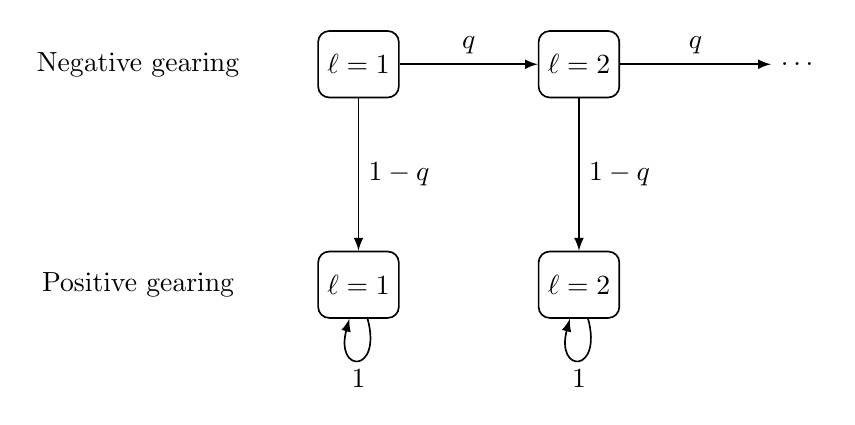
\begin{tikzpicture}[-latex, auto, node distance = 2.8cm, on grid, semithick, state/.style = {draw, rounded corners, minimum height = 24pt}, every loop/.style={-latex}]
\node[state] (1) {$\ell = 1$};
\node[left of = 1, align = right] (0) {Negative gearing};
\node[state, below of = 1] (2) {$\ell = 1$};
\node[left of = 2, align = right] (0A) {Positive gearing};
\node[state, right of = 1] (3) {$\ell = 2$};
\node[right of = 3] (dot1) {\dots};
\node[state, below of = 3] (4) {$\ell = 2$};

\path (1) edge node[anchor = south]{$q$} (3);
\path (1) edge node[anchor = west]{$1 - q$}(2);
\path (3) edge node[anchor = south]{$q$} (dot1);
\path (3) edge node[anchor = west]{$1 - q$}(4);

\path (2) edge[loop below] node[anchor=north]{$1$} (2L);
\path (4) edge[loop below] node[anchor=north]{$1$} (4L);
\end{tikzpicture}
\end{figure*}

\begin{figure*}
\Caption{Positive gearing absorbing, age-based ($MA$)}{Diagram of model. $q_x = {}$ probability of negatively gearing, given a property investor at age $x$}{fig:Markov-MA}
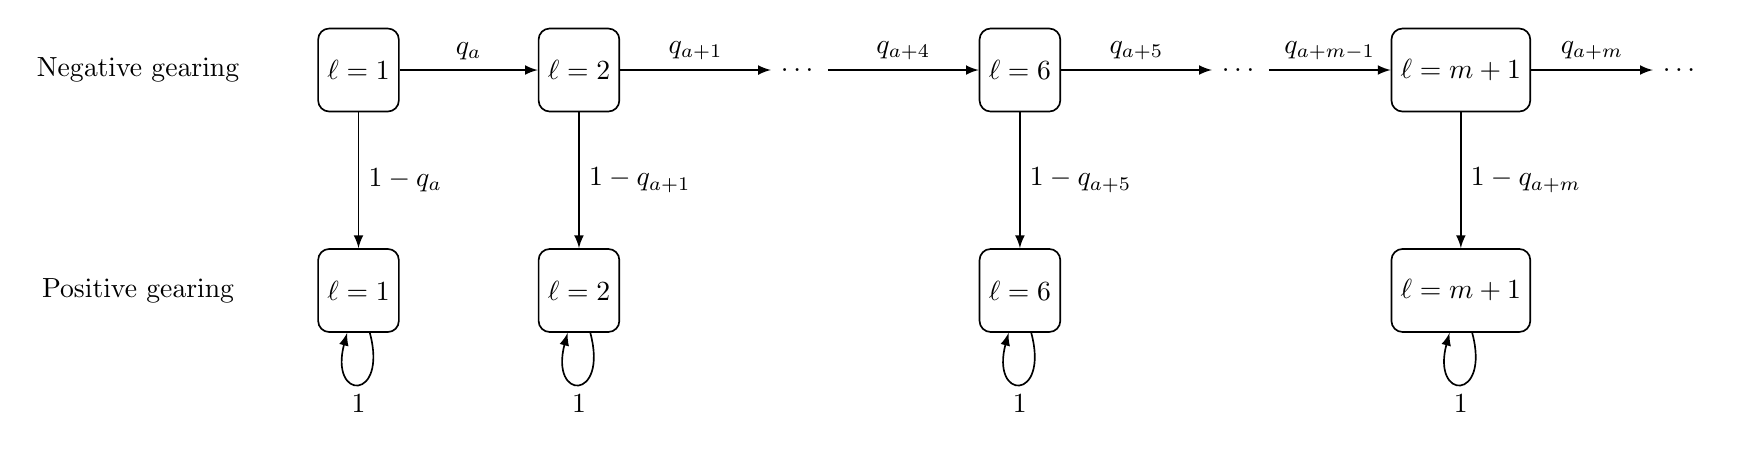
\begin{tikzpicture}[-latex, auto, node distance = 2.8cm, on grid, semithick, state/.style = {draw, rounded corners, minimum height = 30pt}, every loop/.style={-latex}]
\node[state] (1) {$\ell = 1$};
\node[left of = 1, align = right] (0) {Negative gearing};
\node[state, below of = 1] (2) {$\ell = 1$};
\node[left of = 2, align = right] (0A) {Positive gearing};
\node[state, right of = 1] (3) {$\ell = 2$};
\node[right of = 3] (dot1) {\dots};
\node[state, below of = 3] (4) {$\ell = 2$};

\path (1) edge node[anchor = south]{$q_a$} (3);
\path (1) edge node[anchor = west]{$1 - q_a$}(2);
\path (3) edge node[anchor = south]{$q_{a + 1}$} (dot1);
\path (3) edge node[anchor = west]{$1 - q_{a + 1}$}(4);

\path (2) edge[loop below] node[anchor=north]{$1$} (2L);
\path (4) edge[loop below] node[anchor=north]{$1$} (4L);

\node[state, right of = dot1] (6) {$\ell = 6$};
\node[state, below of = 6] (7) {$\ell = 6$}; 
\node[right of = 6] (dot2) {\dots};
\node[state, right of = dot2] (11) {$\ell = m + 1$};
\node[state, below of = 11] (12) {$\ell = m + 1$};
\node[right of = 11] (dot3) {\dots};

\path (dot1) edge node[anchor = south]{$q_{a + 4}$} (6);

\path (6) edge node[anchor = south]{$q_{a + 5}$} (dot2);
\path (6) edge node[anchor = west]{$1 - q_{a + 5}$}(7);

\path (7) edge[loop below] node[anchor=north]{$1$} (7L);

\path (dot2) edge node[anchor = south]{$q_{a + m - 1}$} (11);
\path (11) edge node[anchor = south]{$q_{a + m}$} (dot3);
\path (11) edge node[anchor = west]{$1 - q_{a + m}$} (12);

\path (12) edge[loop below] node[anchor=north]{$1$} (12L);
\end{tikzpicture}

\notes{$q_i = q_j$ for all $i,j \in \{a, a + 1, \dots, a + 4\}$ when $a = 0\mod 5$.}
\end{figure*}


% citations
\nocite{R-sessioninfo,R-bindrcpp,R-hildaData,R-ggrepel,R-testthat,R-hutils,R-taxstats1516,R-taxstats,R-magrittr,R-tidyr,R-usethis,R-devtools,R-expm,R-Hmisc,R-Formula,R-lattice,R-foreign,R-survey,R-survival,R-Matrix,R-zoo,R-httr,R-rsdmx,R-readr,R-openxlsx,R-readxl,R-xtable,R-grattan,R-directlabels,R-scales,R-ggplot2,R-gridExtra,R-dplyr,R-data.table,R-haven,R-hutilscpp,R-grattanCharts,R-knitr}







\end{document}
